\chapter{Orbital dynamics around Asteroids}
\label{chap:dynamics_modeling}
\graphicspath{{Modeling/Images/}}

This chapter will focus on accurate modeling of the asteroid environment and the equations of motion of a particle around it in presence of gravitational and Solar perturbations.

\section{Modeling Assumptions}
\label{sec:assumptions}
The simulator designed as part of this research (see \Cref{chap:naos}) involves some degree of approximation of the real-world dynamical environment around the asteroid. Every degree-of-freedom and complexity added to a simulator to resemble the real-world, will also act as a potential source of error. By designing a relatively simpler simulator, we can explain the characteristic behavior of regolith through fundamentals while keeping the sources of error to as low as possible. Ofcourse, we verify the simulator (see \Cref{chap:v_and_v}) but by including a higher degree of fidelity in the simulator, we increase the workload on the verification process as well, thereby reducing the scientific output in the end. Moreover, the current simulator and the results from it will act as a benchmark for a higher-fidelity simulator in the future. Thus, the approximations made in this thesis are mentioned as follows:
% Every research involves some degree of approximation of the natural world, on Earth or otherwise, to understand or explain any phenomenon. Through this thesis work, we hope to understand the orbital behavior of regolith around an asteroid and we have to do it with a relatively simplified model because recreating an exact replica of an asteroid's dynamical environment is out of the scope of this thesis. Although we are making simplifications, but it does not mean that the scientific returns from it would be any less. The particle trajectories might not be exact when we conduct the simulation based experiments in real world but the underlying science explaining the orbital behavior would remain unchanged (this would become more clear in \Cref{chap:results}). Thus, the simplifying assumptions we make for modeling the asteroid-regolith system are mentioned as follows:
%%%
\begin{enumerate}
\item The asteroid body is modeled as a smooth triaxial ellipsoid to account for its non-uniform gravity. The triaxial model is chosen over the spherical and ellipsoidal harmonics approach because we want to study motion of regolith close to the surface of the asteroid; in particular the re-impact scenarios. This can't be done with the harmonics model as the gravitational potential diverges, within the circumscribing volume, from the true potential of an irregular body (see \Cref{sec:gravity}). We chose not to use a polyhedron model either, even though it can account for surface irregularities of an irregular body much better than the triaxial ellipsoid. This is because we want to decouple the fundamental phenomenon, associated with the motion of the regolith, from any effects of a truly irregular shape such as in the case of a polyhedron model.

\item Craters, surface depressions, mountains or any other terrain deformity on the asteroid is not considered in the simulation. The body is considered to have a uniform density. This is to simplify calculations of the gravitational acceleration.

\item The asteroid is rotating uniformly about its shortest axis. This is considered for simplicity and also because most Solar System bodies would dissipate energy to eventually enter a rotational state that is uniform and about its axis of maximum moment of inertia \parencite{scheeresBook}. Hence, the approximation for the asteroid remains valid.

\item The regolith grains are assumed to be spherical in shape to simplify the \gls{SRP} calculation as the cross-sectional area of a sphere would remain the same irrespective of its attitude. In addition to this, the grains are assumed to have albedo equal to one which means that any impinging Solar photons are completely reflected and this is done to account for maximum perturbation from \gls{SRP} for a given location and Area-To-Mass ratio (see \Cref{subsec:srp} for more details).

\item Multiple regolith particles are launched from a given location on the asteroid in the form of a cone to replicate ejecta from a cratering event. But all particles are assumed to be coming off from the same point, unlike that in the case of an actual cratering event. This is because the pretext of the thesis was that the regolith is lofted due to an activity from a spacecraft and such would result in relatively smaller craters (from artificial cratering events) or surface depressions. Thus assuming that all particles in this \textit{"ejecta cone"} emerge from the same point on the asteroid is reasonable and simplifies the simulation.

\item The slant angle of the \textit{"ejecta cone"} (henceforth the declination angle) from the local surface normal is kept constant at \SI{45.0}{\degree} (which is a middle value in the entire declination range from \SI{0.0}{\degree} - \SI{90.0}{\degree}). We want to consider a general case and not introduce another degree-of-freedom in terms of varying declination angles.

\item The loss of material and mass from the asteroid, when the regolith is lofted from the surface, is not modeled in the simulation since it is assumed that a very small amount of material will be displaced by a spacecraft activity. This assumption is based on the sample collected by the Hayabusa mission (see \Cref{sec:past_missions} and the references therein).

\item Interaction between individual regolith grain is not accounted for because we are simulating multiple particles being lofted at the same time and granular interaction on such a scale would be extremely complex and beyond the scope of this thesis.

\item Secondary motion of regolith, after re-impacting the surface is not modeled and it is assumed that the particles just come to a standstill.

\item The shadow region of the asteroid is not modeled which means that the solar perturbations are always acting on the regolith grain and this simplification was made since asteroids are extremely small compared to planets, and thus the orbiting particles wouldn't spend long periods of time in the shadow.

\item Perturbations are considered only from the Sun. \gls{SRP} is important because regolith grains will have higher Area-To-Mass ratios, relative to a spacecraft, and so the radiation pressure would be significantly large for them. We model the third body attraction from the Sun (\gls{STBE}) as well but not from any of the planets because we are assuming that the small body does not pass close to any planet, thus rendering the perturbations from them insignificant.
% The magnitude of perturbation from the \gls{STBE} itself is atleast 5 orders of magnitude smaller than the gravitational acceleration (for a sample asteroid assumed to be in a circular orbit at 1 AU from the Sun) when the regolith is in close proximity to the asteroid (see \Cref{chap:results}).

\item The apparent motion of the Sun around the asteroid is considered circular and in the equatorial plane of the asteroid and this was based on the orbital element measurements of all observed asteroids. Majority of these asteroids have small orbital eccentricities \parencite{malhotra2016_eccentricityDistribution}, quite a few of which have a nearly circular orbit. \cite{jedicke1998_orbitalElements} presents debiased measurements for the inclination of the \gls{MBO} and shows that a large number of asteroids have near-zero inclinations.
\end{enumerate}
%%%
\newpage
\section{Reference Frames}
\label{sec:reference_frames}
Before describing the motion of regolith around the asteroid, its important to define the frames of reference with respect to which this motion is defined and the transformation of state vectors between these frames. We use two asteroid centric reference frames, both of which are depicted in \Cref{fig:reference_frame}. Since we will be using a triaxial ellipsoid to model an asteroid (for details, see \Cref{sec:gravity}), the body-fixed rotating frame and the inertial frame with respect to this model are shown in \Cref{fig:ellipsoid_rotating_frame,fig:solar_phase_and_inertial_frame} respectively.
%%%
\begin{figure}[htb]
\centering
\captionsetup{justification=centering}
\includegraphics[width=\textwidth, height=0.30\textheight, keepaspectratio=true]{reference_frames.pdf}
\caption{The diagram depicts two asteroid centric reference frames, one being Inertial (depicted by solid line and the subscript \emph{I}) and the other being a body-fixed Rotating frame (denoted by dashed line and the subscript \emph{B}). The position vector to a regolith particle is shown as $\protect\vv{\bm{r}}_{P,B}$, whereas the position vector to the Sun from the asteroid is shown as $\protect\vv{\bm{r}}_{S,I}$.}
\label{fig:reference_frame}
\end{figure}
\FloatBarrier
%%%
The two frames are defined as follows:
%%%
\begin{enumerate}
\item \gls{AIF} - This is a non-rotating frame fixed inertially in space with its origin at the centre of mass of the asteroid . \Cref{fig:solar_phase_and_inertial_frame} shows the orientation of the frame (in \emph{x-y} plane) such that the \emph{x-axis} is pointing to the Sun when the Longitude of the Sun (or effectively the True Anomaly of the apparent circular motion of the Sun around the asteroid) $\vartheta$ is zero. The \emph{y-axis}, thus, points to the sun when $\vartheta = 90^o$ and finally the \emph{z-axis} is obtained by following the right-hand rule, coming out of the sheet in 3D.
%
\item \gls{ARF} - This frame is fixed to the rotating asteroid with its origin at the centre of mass of the asteroid and axes aligned with the principle axes of the asteroid. \Cref{fig:ellipsoid_rotating_frame} shows the orientation of this frame, assuming a triaxial ellipsoid model for our asteroid (for details see \Cref{sec:gravity}). The \emph{x-axis} is pointing along the longest axis of the triaxial ellipsoid, and the \emph{z-axis} is pointing along the shortest axis of the ellipsoid. It is also aligned with the $z_I$ axis of \gls{AIF} as shown in \Cref{fig:reference_frame}. The \emph{y-axis} points in the direction of the remaining third axis, satisfying the right-hand rule. The asteroid (and effectively the \gls{ARF}) is rotating in a counter-clockwise sense, with respect to the \gls{AIF}, with constant angular velocity $\omega$ about the $z_B$ axis as depicted in \Cref{fig:reference_frame}.
\end{enumerate}
%%%
%%%
\begin{figure}[htb]
\centering
\captionsetup{justification=centering}
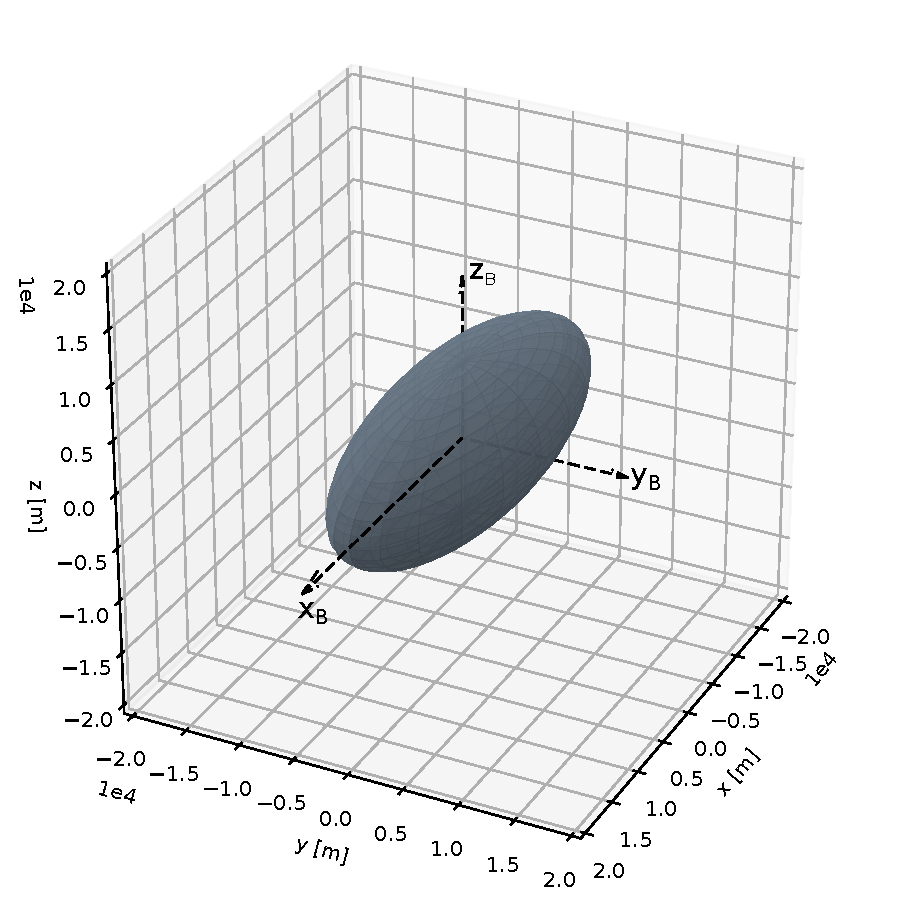
\includegraphics[width=\textwidth, height=0.35\textheight, keepaspectratio=true]{body_fixed_ellipsoid_frame.pdf}
\caption{Representation of the body-fixed rotating frame for a triaxial ellipsoid model of an asteroid. $\bm{x_{B}}$ is aligned with the longest axis, $\bm{z_{B}}$ is aligned with the shortest axis and $\bm{y_{B}}$ is aligned with the remaining last axis of the ellipsoid, satisfying the right-hand rule.}
\label{fig:ellipsoid_rotating_frame}
\end{figure}
\FloatBarrier
%%%
%%%
\begin{figure}[htb]
\centering
\captionsetup{justification=centering}
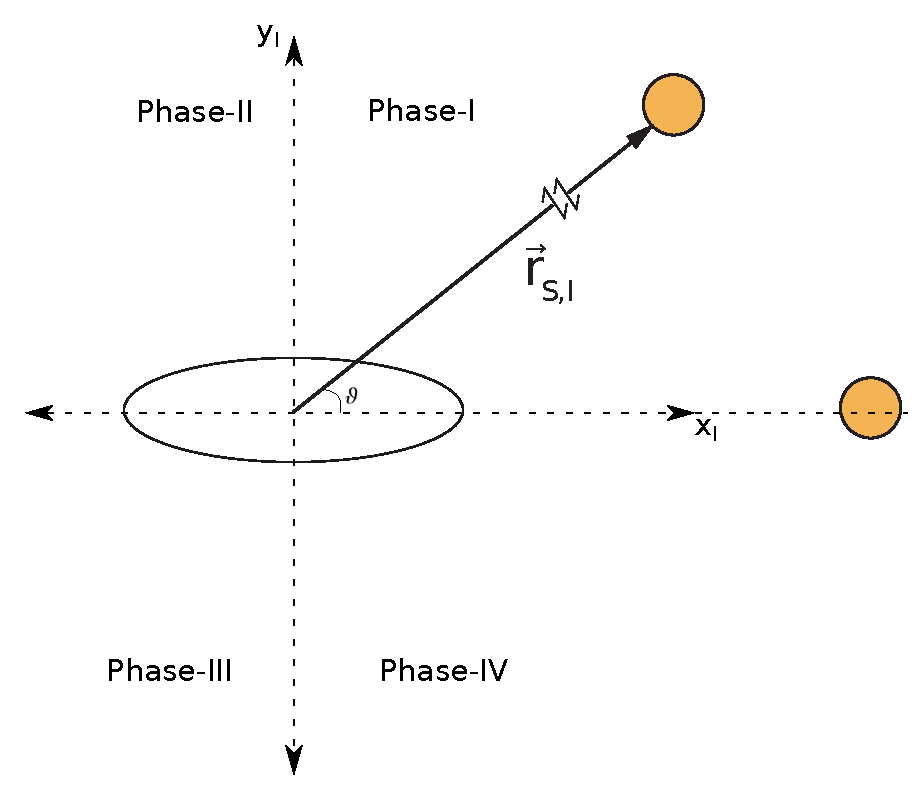
\includegraphics[width=\textwidth, height=0.35\textheight, keepaspectratio=true]{solar_phase_and_inertial_frame_3.pdf}
\caption{Asteroid-centric inertial frame \emph{x-y} plane. The position vector to the Sun is shown as $\protect\vv{\bm{r}}_{S,I}$. The apparent motion of the Sun around the asteroid, assumed a circular orbit, is also depicted with $\vartheta$ as the Longitude of Sun (or effectively the True Anomaly). The four phases are for a broader identification of the Sun's location with respect to the asteroid.}
\label{fig:solar_phase_and_inertial_frame}
\end{figure}
\FloatBarrier
%%%
We have two different frames of reference because it is important to visualize the same orbital motion with respect to both an inertial frame and a non-inertial frame to get a better understanding of the underlying dynamics. In this regard, it is thus important to be able to transfer a state vector between the two frames. The transfer matrix to transform a state vector from \gls{ARF} to \gls{AIF} is given as follows \parencite{schaub2003Book}:
%%%
\begin{equation}
    \begin{aligned}
        \phi_{B}^{I} &=
        \begin{bmatrix}
            \cos\theta & -\sin\theta & 0 \\
            \sin\theta & \cos\theta & 0 \\
            0 & 0 & 1
        \end{bmatrix}
        \\
        \theta &= \omega t
    \end{aligned}
    \label{eqn:arf_to_aif_transformation matrix}
\end{equation}
%%%
In \Cref{eqn:arf_to_aif_transformation matrix}, $\theta$ is the angle of rotation between the \gls{ARF} and the \gls{AIF} at any given time $t$; and $\omega$ is the constant angular velocity of the rotating asteroid about $z_I / z_B$ axis as shown in \Cref{fig:reference_frame}. The position vector is then transformed, from \gls{ARF} to \gls{AIF}, as follows \parencite{schaub2003Book}:
%%%
\begin{align}
    \begin{bmatrix}
        x_I \\
        y_I \\
        z_I
    \end{bmatrix}
    =
    \begin{bmatrix}
        \cos\theta & -\sin\theta & 0 \\
        \sin\theta & \cos\theta & 0 \\
        0 & 0 & 1
    \end{bmatrix}
    \begin{bmatrix}
        x_B \\
        y_B \\
        z_B
    \end{bmatrix}
    \label{eqn:arf_to_aif_position_transformation}
\end{align}
%%%
In \Cref{eqn:arf_to_aif_position_transformation}, $x_I$ and $x_B$ are the x-components of the position vector in \gls{AIF} and \gls{ARF} respectively; other components follow similar definitions. The velocity transformation takes place by first using the \textit{transport theorem} and then multiplying the resultant with the transformation matrix $\phi_{B}^{I}$ \parencite{schaub2003Book}. The transformation is shown as follows:
%%%
\begin{align}
    \vv{\bm{v}}_{I}^{B} &= \vv{\bm{v}}_{B} + \vv{\bm{\omega}} \times \vv{\bm{r}}_{B}
    \label{eqn:arf_to_aif_transport_theorem} \\
    \vv{\bm{v}}_I &= \phi_B^I \vv{\bm{v}}_I^B
    \label{eqn:arf_to_aif_velocity_transformation}
\end{align}
%%%
\Cref{eqn:arf_to_aif_transport_theorem} is the application of the transport theorem to get the \gls{AIF} velocity in \gls{ARF} components ($\vv{\bm{v}}_{I}^{B}$). In that, $\vv{\bm{v}}_{B}$ is the velocity vector in the \gls{ARF}, $\vv{\bm{\omega}}$ is the angular velocity vector for the asteroid's rotation (note that we have only uniform rotation about the $z_B$ axis), and $\vv{\bm{r}}_{B}$ is the position vector defined in the \gls{ARF}. In \Cref{eqn:arf_to_aif_velocity_transformation}, $\vv{\bm{v}}_I$ is the velocity vector in the \gls{AIF}.
%
\newline\newline
%
The transfer matrix to transform a state vector from \gls{AIF} to \gls{ARF} is just the transpose of $\phi_B^I$ as it is orthogonal \parencite{schaub2003Book}. It is given as follows:
%%%
\begin{align}
    \phi_{I}^{B} &=
    \begin{bmatrix}
        \cos\theta & \sin\theta & 0 \\
        -\sin\theta & \cos\theta & 0 \\
        0 & 0 & 1
    \end{bmatrix}
    \label{eqn:aif_to_arf_transformation matrix}
\end{align}
%%%
Then the state vector transformation from \gls{AIF} to \gls{ARF} takes place as follows:
%%%
\begin{align}
    \bvector{r}_B &= \phi_I^B \bvector{r}_I
    \label{eqn:aif_to_arf_position} \\
    \bvector{v}_B^I &= \bvector{v}_I - \bvector{\omega} \times \bvector{r}_I
    \label{eqn:aif_to_arf_transport_theorem} \\
    \bvector{v}_B &= \phi_I^B \bvector{v}_B^I
    \label{eqn:aif_to_arf_velocity}
\end{align}
%%%
where $\bvector{v}_B^I$ is the \gls{ARF} velocity in \gls{AIF} components, and $\bvector{r}_I$ is the position vector in the \gls{AIF}.

\section{Gravitational Potential}
\label{sec:gravity}
% ...elliptic integral method and how the accelerations are calculated and the third order equation solving for lambda...
The key feature that differentiates small bodies, or asteroids for our particular case, from planets is their highly irregular shapes and thus non-spherical mass distributions \parencite{scheeresBook}. This is why the dynamics close to an asteroid are deemed as interesting and hence it is very important that the gravitational potential is modeled properly.

\subsection{Spherical and Ellipsoidal Harmonics}
\label{subsec:spherical_ellipsoidal_harmonics}
One of the most common methods for modeling gravity potential of any celestial body is the \textit{spherical harmonics} model. In that, a sphere whose radius is equal to the maximum dimension of the irregular body, circumscribes it and this sphere is called the \textit{Brillouin sphere} (see \Cref{fig:brillouin_sphere}). The spherical harmonics model then induces deformities on the Brillouin sphere, thereby producing a non-spherical gravity field. The spherical harmonics gravity potential is stated as follows \parencite{scheeresBook}:
%%%
\begin{align}
    U(r, \delta, \lambda) = \frac{\mu}{r} \sum_{l=0}^{\infty} \sum_{m=0}^{l} \left(\frac{r_0}{r}\right)^l P_{lm} (\sin\delta) [C_{lm}\cos m\lambda + S_{lm}\sin m\lambda]
    \label{eqn:spherical_harmonics_general}
\end{align}
%%%
where $U$ is the gravitational potential calculated at a distance $r$ from the centre of the Brillouin sphere at latitude $\delta$ and longitude $\lambda$, $\mu$ is the gravitational parameter of the irregular body or asteroid, $r_0$ is the radius of the Brillouin sphere, $P_{lm}$ are the associated Legendre functions, $C_{lm}$ and $S_{lm}$ are the spherical harmonic coefficients which account for shape and density variations \parencite{romain2001ellipsoidal}, and $l$ and $m$ are the degree and order, respectively, of the spherical harmonic expansion. The definitions and calculations for the associated Legendre functions and the harmonics coefficients has been explained in detail by \cite{scheeresBook} and is not repeated here for brevity. The majority of gravity field perturbations can be accounted for by just considering the second degree and order in the spherical harmonics expansion. The potential is then expressed as follows \parencite{scheeresBook}:
%%%
\begin{align}
    U = \frac{\mu}{r} \left[ 1 + \left(\frac{r_0}{r}\right)^2 \left\{C_{20} \left(1-\frac{3}{2}\cos^2\delta\right) + 3C_{22}\cos^2\delta \cos(2\lambda) \right\} \right]
    \label{eqn:spherical_harmonics_second_degree}
\end{align}
%%%
where the spherical harmonic coefficients can be obtained from the principle moments of inertia as defined in \cite{scheeresBook}.
%%%
\begin{figure}[htb]
\centering
\captionsetup{justification=centering}
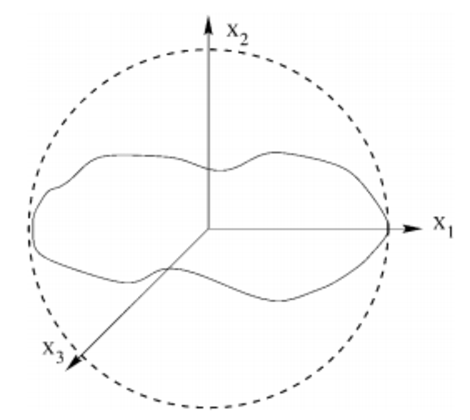
\includegraphics[width=\textwidth, height=0.25\textheight, keepaspectratio=true]{Brillouin_sphere.pdf}
\caption{Brillouin sphere or the circumscribing sphere around an irregular body \parencite{romain2001ellipsoidal}.}
\label{fig:brillouin_sphere}
\end{figure}
\FloatBarrier
%%%
Now consider a general statement for the gravity field of any arbitrary mass distribution $\mathcal{B}$ \parencite{scheeresBook}:
%%%
\begin{align}
    U = \frac{\mu}{V} \int_{\mathcal{B}} \frac{dV}{|\bvector{r} - \bvector{\rho}|}
    \label{eqn:general_gravity_field}
\end{align}
%%%
where $V$ is the volume, $\bvector{r}$ is the position vector to the point where the potential is being calculated, $\bvector{\rho}$ is the position vector to the discrete mass distribution within $\mathcal{B}$. If the potential is being calculated for a point that lies outside the maximum radius of the mass distribution being considered, then the integrand in \Cref{eqn:general_gravity_field} can be expanded into the following Laplace series form \parencite{scheeresBook}:
%%%
\begin{align}
    \frac{1}{|\bvector{r} - \bvector{\rho}|} = \frac{1}{r} \sum_{i=0}^{\infty} \left(\frac{\rho}{r}\right)^i P_{i0} \left(\frac{\bvector{r} \cdot \bvector{\rho}}{r\rho}\right)
    \label{eqn:general_grav_term_laplace_series}
\end{align}
%%%
where $P_{i0}$ are the Legendre polynomials. Thus using \Cref{eqn:general_grav_term_laplace_series}, the integral in \Cref{eqn:general_gravity_field} can be restated as follows \parencite{scheeresBook}:
%%%
\begin{align}
    \frac{1}{V} \int_{\mathcal{B}} \left(\frac{\rho}{r}\right)^i P_{i0} \left(\frac{\bvector{r} \cdot \bvector{\rho}}{r\rho}\right) dV
    \label{eqn:general_gravity_field_modified_integral}
\end{align}
%%%
There is a one-to-one correspondence between the integral in \Cref{eqn:general_gravity_field_modified_integral} and the $i$th degree and order spherical harmonics gravity field. Thus by looking at the Laplace series in \Cref{eqn:general_grav_term_laplace_series} and the integral in \Cref{eqn:general_gravity_field_modified_integral}, we can infer on the convergence or divergence of the spherical harmonics gravity field. Since the maximum radius of the mass distribution in case of the spherical harmonics model would be that of the circumscribing or Brillouin sphere, then for a point on this sphere, i.e. $r = |\bvector{\rho}|$, the Laplace series is not defined and for a point inside the sphere, i.e. $r < |\bvector{\rho}|$, the Laplace series diverges. This is the limitation for using the spherical harmonics model for an irregular body when one wants to compute orbital motion in close-proximity to the body. If the computation points are within the Brillouin sphere then the spherical harmonics series might diverge to a value that does not represent the true gravitational potential value and hence lead to errors in orbit computations. We can see from \Cref{fig:brillouin_sphere} that the volume of divergence for irregularly shaped asteroids can be quite significant. Thus, this model is definitely not suitable for our research since we are dealing with close-proximity orbits and above all, particle re-impact scenarios.
%%%
\begin{figure}[htb]
\centering
\captionsetup{justification=centering}
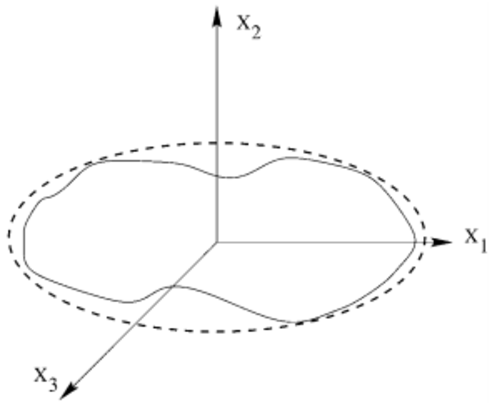
\includegraphics[width=\textwidth, height=0.25\textheight, keepaspectratio=true]{Brillouin_ellipsoid.pdf}
\caption{Brillouin ellipsoid or the circumscribing ellipsoid around an irregular body \parencite{romain2001ellipsoidal}.}
\label{fig:brillouin_ellipsoid}
\end{figure}
\FloatBarrier
%%%
The above problem can be mitigated, to a certain extent, by using the \textit{ellipsoidal harmonics} expansion for representing the gravity potential of an irregular body. An extremely detail account on this model is given by \cite{dechambre2002transformation}. In the ellipsoidal harmonics model, instead of a sphere, a triaxial ellipsoid is used to circumscribe the irregular body and proves to be a better fit as shown in \Cref{fig:brillouin_ellipsoid}. The ellipsoidal harmonics potential is then given as follows \parencite{dechambre2002transformation}:
%%%
\begin{align}
    U(\lambda_1, \lambda_2, \lambda_3) &= \mu \sum_{n=0}^{\infty} \sum_{p=1}^{2n+1} \alpha_{np} \frac{E_n^p(\lambda_1)}{E_n^p(\lambda_1^{ref})} \times E_n^p(\lambda_2) E_n^p(\lambda_3) \text{; $\lambda_1 \leq \lambda_1^{ref}$}
    \label{eqn:ellipsoidal_harmonics_inside} \\
    U(\lambda_1, \lambda_2, \lambda_3) &= \mu \sum_{n=0}^{\infty} \sum_{p=1}^{2n+1} \alpha_{np} \frac{F_n^p(\lambda_1)}{F_n^p(\lambda_1^{ref})} \times E_n^p(\lambda_2) E_n^p(\lambda_3) \text{; $\lambda_1 \geq \lambda_1^{ref}$}
    \label{eqn:ellipsoidal_harmonics_outside}
\end{align}
%%%
where $(\lambda_1, \lambda_2, \lambda_3)$ are the ellipsoidal coordinates, which are basically three real roots (solutions) in terms of $s$ for the following conic equation \parencite{garmier2002modeling}:
%%%
\begin{align}
    \frac{x^2}{s^2 + a^2} + \frac{y^2}{s^2 + b^2} + \frac{z^2}{s^2 + c^2} = 1
    \label{eqn:conic_ellipsoidal}
\end{align}
%%%
where $(x, y, z)$ are the Cartesian coordinates and $(a, b, c)$ are the semi-major axes of the reference ellipsoid circumscribing the irregular body (note that $a=\lambda_1^{ref}$). In \Cref{eqn:ellipsoidal_harmonics_inside,eqn:ellipsoidal_harmonics_outside}, $(\lambda_1, \lambda_2, \lambda_3)$ are analogous to the radius $r$, latitude $\delta$ and longitude $\lambda$, respectively, of \Cref{eqn:spherical_harmonics_general}; $\alpha_{np}$ is the ellipsoidal harmonics expansion coefficient similar to the spherical harmonics coefficient $C_{lm}$ and $S_{lm}$; $F_n^p()$ are the Lam\'e function of second kind of degree $n$ and order $p$ and is analogous to the attenuation term $(r_0 / r)^l$ of the spherical harmonics expansion in \Cref{eqn:spherical_harmonics_general}; $E_{n}^p()$ is the Lam\'e function of the first kind of degree $n$ and order $p$; and finally, the product term $E_{n}^p(\lambda_2)E_{n}^p(\lambda_3)$ is analogous to the product term $P_{lm} (\sin\delta) [C_{lm}\cos m\lambda + S_{lm}\sin m\lambda]$ which in both cases models the surface harmonic \parencite{garmier2002modeling}. A detailed description on definition and calculation of the ellipsoidal harmonic coefficients and the Lam\'e functions of the first and the second kind can be found in \cite{dechambre2002transformation} and is not repeated here for brevity.
%
\newline\newline
%
Even in the case of ellipsoidal harmonics expansion model, the gravity potential calculated for a point inside the circumscribing ellipsoid can diverge from the true potential. But the advantage of this model over the spherical harmonics expansion is that the circumscribing reference ellipsoid reduces the volume of divergence around the irregular body, relative to a sphere, making close-proximity evaluations possible. However, relative to spherical harmonics expansion, the computation of the basis functions for ellipsoidal harmonics, i.e. the Lam\'e functions of the first and the second kind, is extremely complex. On top of that, with increasing degree of the harmonics model, the order of magnitude of the Lam\'e functions increases, which then runs the risk of arithmetic overflow, thereby impeding accurate calculations of the harmonic expansion for degrees above 10 to 15 \parencite{reimond2016spheroidal}. However, in their research, \cite{reimond2016spheroidal} have devised a new method to calculate the basis functions using logarithmic expressions which allows accurate harmonic expansions for degrees of upto 500 but the computational complexity also increases tremendously as stated by them. Ultimately, since we wish to express the motion of particles close to the surface of the asteroid, which also involves surface interactions, the approach of ellipsoidal harmonics expansion also fails.

\subsection{Constant Density Polyhedron}
\label{subsec:polyhedron}
The gravity potential modeling methods discussed so far involved the use of surface harmonics on the circumscribing object (sphere or ellipsoid) to simulate a non-homogeneous gravity field for an irregular body. The major drawback with the harmonics approach was its divergence from the true potential value within the circumscribing volume. This problem can be mitigated all together by assuming a specific shape and density distribution for the irregular body in question. In this realm, there are the \gls{CDE} and constant density polyhedron gravity potential models. Unlike the harmonics expansion approach, these potential models are valid upto and on the surface of the shape that has been assumed for the irregular body in question \parencite{scheeresBook}. Hence, these models are perfect to study close-proximity motion of particles or spacecraft around an asteroid.
%
\newline\newline
%
The irregular shape of an asteroid can be best represented by a polyhedron shape model (henceforth polyhedron) as shown in \Cref{fig:polyhedron_example}. Surface irregularities in the form of craters, large boulders, mountains etc. can be easily modeled with this method. A polyhedron is basically a 3D body that consists of several \textit{vertices} which form triangular faces or \textit{facets} that are connected to each other through the \textit{edges} of each face. A triangular facet thus comprises of three vertices, three edges and a surface normal as shown in \Cref{fig:single_facet} \parencite{scheeresBook}. A detailed derivation for the polyhedron gravitational potential model is given in \cite{scheeres_polyhedra} and concisely presented in \cite{scheeresBook} as well. Hence, we will only present a summary of this method in this section.
%%%
\begin{figure}[htb]
\centering
\captionsetup{justification=centering}
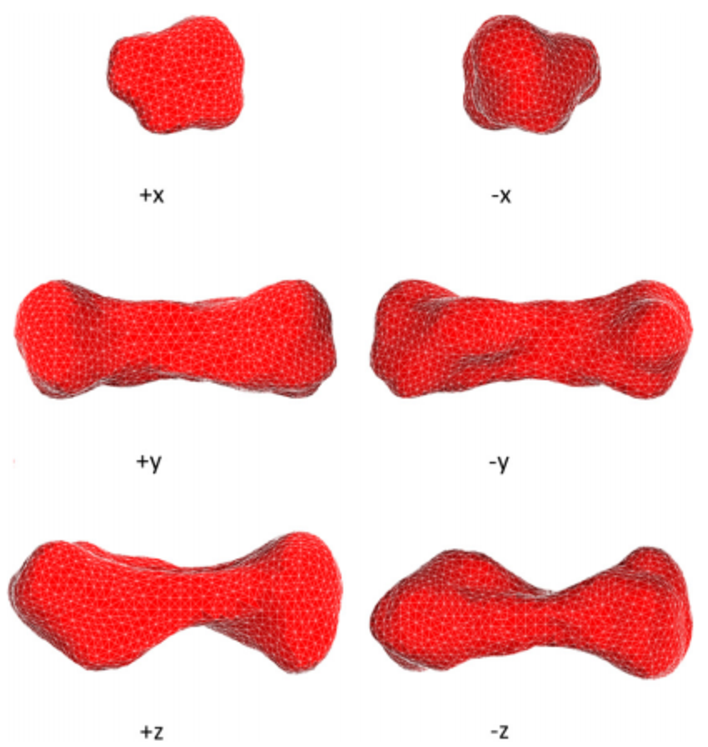
\includegraphics[width=\textwidth, height=0.3\textheight, keepaspectratio=true]{polyhedra_example.pdf}
\caption{Polyhedron shape model estimated for asteroid \textit{Kleopatra} and shown in $\pm x, \pm y, \pm z$ axis directions. Constant density has been assumed in this modeling process. Surface deformities are easily modeled by this method \parencite{polyhedra_example}.}
\label{fig:polyhedron_example}
\end{figure}
\FloatBarrier
%%%
%%%
\begin{figure}[htb]
\centering
\captionsetup{justification=centering}
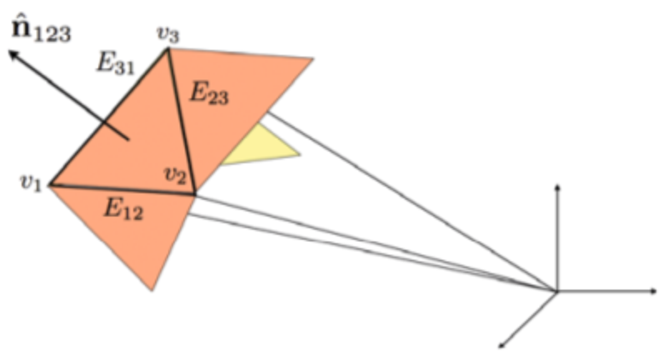
\includegraphics[width=\textwidth, height=0.2\textheight, keepaspectratio=true]{single_facet.pdf}
\caption{Single facet of a polyhedron model depicting three vertices, three edges and a surface normal, associated with each facet in general \parencite{scheeresBook}.}
\label{fig:single_facet}
\end{figure}
\FloatBarrier
%%%
Each face or facet \textit{'f'} of the polyhedron is associated with three vertex vectors given as $\bvector{r}_i^f$, where $i=1,2,3$, and a unit normal vector $\buvec{n}_f$. The vector $\bv{r}_i^f$ goes from each vertex of a facet to the field point \textbf{P} where the potential has to be calculated. Each edge \textit{'e'} is associated to two vertex vectors $\bvector{r}_i^e$, for $i=1,2$, and this edge connects two adjacent faces \textit{f} and \textit{f'}. Again, the vector $\bv{r}_i^e$ goes from the edge vertices to the field point \textbf{P}. The edge normal, corresponding to facet \textit{f}, is denoted as $\buvec{n}_e^f$ such that it is perpendicular to the edge and the facet normal $\buvec{n}_f$ and is pointing away from the centre of the facet. For the same edge shared by facet \textit{f'}, the edge normal $\buvec{n}_e^{f'}$ points in a different direction than $\buvec{n}_e^f$ and may not be parallel to it. With these definitions, the general formula for the polyhedron gravitational potential is given as follows \parencite{scheeresBook}:
%%%
\begin{align}
    U(\bvector{r}) &= \frac{\mathcal{G}\sigma}{2} \left[ \sum_{e\in edges} \bvector{r}_e \cdotp \bm{E}_e \cdotp \bvector{r}_e L_e - \sum_{f\in faces} \bvector{r}_f \cdotp \bm{F}_f \cdotp \bvector{r}_f \omega_f \right]
    \label{eqn:polyhedron_potential} \\
    \bm{E}_e &= \buvec{n}_f \buvec{n}_e^f + \buvec{n}_{f'} \buvec{n}_e^{f'}
    \label{eqn:polyhedron_E_term} \\
    \bm{F}_f &= \buvec{n}_f \buvec{n}_f
    \label{eqn:polyhedron_F_term} \\
    L_e &= ln\left(\frac{r_1^e + r_2^e + e_e}{r_1^e + r_2^e - e_e} \right)
    \label{eqn:polyhedron_L_term} \\
    e_e &= |\bvector{r}_1^e - \bvector{r}_2^e|
    \label{eqn:polyhedron_e_term} \\
    \omega_f &= 2 \tan^{-1} \left(\frac{\bv{r}_1^f \cdotp (\bv{r}_2^f \times \bv{r}_3^f)}{r_1^f r_2^f r_3^f + r_1^f(\bv{r}_2^f \cdotp \bv{r}_3^f) + r_2^f(\bv{r}_3^f \cdotp \bv{r}_1^f) + r_3^f(\bv{r}_1^f \cdotp \bv{r}_2^f)} \right)
\end{align}
%%%
where \bvt{r} is the position vector to the field point \textbf{P} from the origin of an asteroid-fixed reference frame; $\mathcal{G}$ is the universal gravitational constant and $\sigma$ is the density of the body being modeled; $\bvector{r}_e$ is the vector from any point along the edge \textit{'e'} to \bvt{r} or the field point \textbf{P} and in the same way $\bvector{r}_f$ denotes a vector from any point on the facet \textit{f} to \bvt{r} \parencite{scheeresBook}; the term $\omega_f$ represents the solid angle subtended by a facet when viewed from the field point \textbf{P}, or alternately, it is the angle subtended by the facet of the polyhedron on to a unit sphere centered at the field point \textbf{P}; $L_e$ is analogous to the potential of a 1D straight \textit{'wire'} and is computed for all facet edges in a polyhedron \parencite{scheeres_polyhedra}; $\bm{E}_e$ is the edge dyad and is expressed as the sum of two outer-products, forming a 3x3 matrix; and finally $\bm{F}_f$ is the facet dyad which is simply the outer-product of the facet normal vector with itself \parencite{scheeres_polyhedra}.
%
\newline\newline
%
The constant density polyhedron gravitational potential model provides a realistic shape for an irregular body by accounting for topographical irregularities, however, the polyhedron model is computationally expensive \parencite{scheeresBook}. This thesis work does not make use of this model, but instead, employs a triaxial ellipsoid to model the gravitational potential (explained in the following section). This is because we wanted to understand the fundamental phenomenon associated with the motion and final fate of regolith in presence of gravity and Solar perturbations. This fundamental phenomenon would be difficult to decouple from other effects of a true irregular body, such as in the case of a polyhedron model and hence it was not used in this thesis. A triaxial ellipsoid itself is a very good approximation of real small body shapes \parencite{broschart2005control} and hence we don't loose out on the validity of explanations for the fundamental features of regolith motion by excluding the polyhedron model.

\subsection{Constant Density Ellipsoid}
\label{subsec:constant_density_ellipsoid}
Consider a \gls{CDE} with semi-major axes $(\alpha, \beta, \gamma)$ such that $\gamma \leq \beta \leq \alpha$. The shape of the triaxial ellipsoid is completely defined by the equation $(x/\alpha)^2 + (y/\beta)^2 + (z/\gamma)^2 \leq 1$. The density of the ellipsoid is assumed to be constant. An example for a \gls{CDE} model is shown in \Cref{fig:cde}.  Then the gravitational potential for a point external to such a body, i.e. \gls{CDE}, is defined by the following equation \parencite{scheeresBook}:
%%%
\begin{align}
    U(\bvector{r}) &= -\frac{3\mu}{4} \int_{\lambda(\bvector{r})}^{\infty} \phi(\bvector{r}, u) \frac{du}{\Delta(u)}
    \label{eqn:ellipsoid_potential_short_form} \\
    \phi(\bvector{r}, u) &= \frac{x^2}{\alpha^2 + u} + \frac{y^2}{\beta^2 + u} + \frac{z^2}{\gamma^2 + u} - 1
    \label{eqn:ellipsoid_potential_phi} \\
    \Delta(u) &= \sqrt{(\alpha^2 + u)(\beta^2 + u)(\gamma^2 + u)}
    \label{eqn:ellipsoid_potential_delta}
\end{align}
%%%
where $\bvector{r}$ is the position vector to the point, external to the \gls{CDE}, and is defined in the \gls{ARF}; $\lambda(\bvector{r})$ is a parameter defined by the equation $\phi(\bvector{r}, \lambda) = 0$, which is a cubic polynomial as shown in \Cref{eqn:cubicPolynomial}, and the value $\lambda$ is the maximum real root of this polynomial \parencite{scheeresBook}.
%%%
\begin{align}
    \lambda^3 &+ \nonumber \\
    \lambda^2 (\alpha^2 + \beta^2 + \gamma^2 - (x^2 + y^2 + z^2)) &+ \nonumber \\
    \lambda (\alpha^2 \beta^2 + \alpha^2 \gamma^2 + \beta^2 \gamma^2 - x^2(\beta^2 + \gamma^2) - y^2(\alpha^2 + \gamma^2) - z^2(\alpha^2 + \beta^2)) &+ \nonumber \\
    (\alpha^2 \beta^2 \gamma^2 - x^2 \gamma^2 \beta^2 - y^2 \alpha^2 \gamma^2 - z^2 \alpha^2 \beta^2) &= 0
    \label{eqn:cubicPolynomial}
\end{align}
%%%
%%%
\begin{figure}[htb]
\centering
\captionsetup{justification=centering}
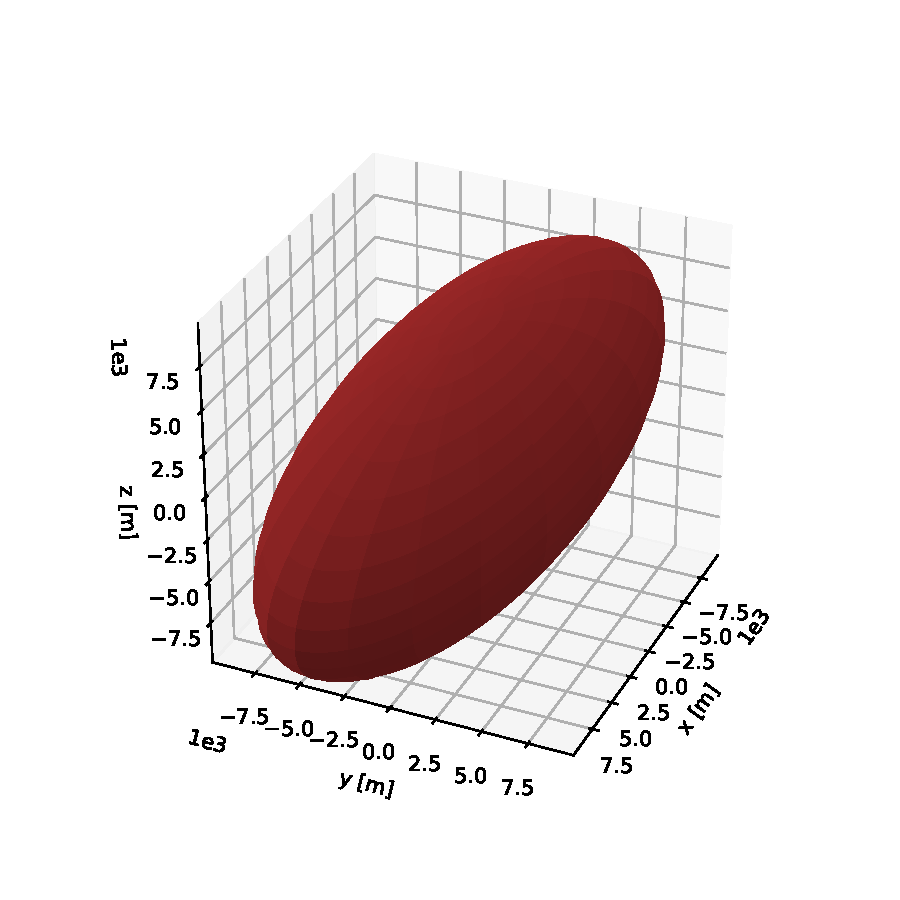
\includegraphics[width=\textwidth, height=0.27\textheight, keepaspectratio=true]{cde.pdf}
\caption{Triaxial ellipsoid model with semi-major axes $\alpha=20$ km, $\beta=7$ km, $\gamma=7$ km.}
\label{fig:cde}
\end{figure}
\FloatBarrier
%%%
For a given point $(x, y, z)$ in space around the \gls{CDE}, the only unknown in \Cref{eqn:cubicPolynomial} is $\lambda$ which is solved for using the standard Cardano's formula (see \cite{cubic_formula}). Now for the given ellipsoid, the equation for the family of confocal quadratic surfaces is given as follows \parencite{ellipsoid_potential_model}:
%%%
\begin{align}
    \frac{x^2}{\alpha^2 + u} + \frac{y^2}{\beta^2 + u} + \frac{z^2}{\gamma^2 + u} &= 1
    \label{eqn:confocal_quadrics}
\end{align}
%%%
where $u$ is a real-valued parameter whose value defines the type of the confocal quadratic surface. \Cref{eqn:confocal_quadrics} is a cubic polynomial in $u$ and can be solved to obtain three unequal real roots - $u_1, u_2, u_3$, such that the following relation holds true \parencite{ellipsoid_potential_model}:
%%%
\begin{align}
    -\alpha^2 < u_3 < -\beta^2 < u_2 < -\gamma^2 < u_1 < +\infty
    \label{eqn:confocal_quadrics_all_real_roots}
\end{align}
%%%
where $u_1$ is the maximum real root possible and at that value, \Cref{eqn:confocal_quadrics} defines another ellipsoid which is confocal to the original one defined by the semi-major axes $\rightarrow$ $\alpha, \beta, \gamma$ \parencite{ellipsoid_potential_model}. Thus, the value of $\lambda$ in \Cref{eqn:ellipsoid_potential_short_form} conforms to a confocal ellipsoid for a given point external to the original ellipsoid (which in turn is modeling the asteroid).
% The standard definition of gravitational potential at a point is defined as the work required to move that point from infinity to the location of the point in question and in \Cref{eqn:ellipsoid_potential_short_form}, this is being done by moving through a family of confocal ellipsoids.
%
\newline\newline
%
The potential defined by \Cref{eqn:ellipsoid_potential_short_form} appears to have a complicated computational process due to its integral form. However, the integral can be split into multiple parts such that each can be solved with the help of standard functions called \textit{Carlson's Elliptic Integrals} \parencite{carlsonEllipticIntegral}. Software routines for these integrals exist in several computing languages which, for our case, helps in computing the \gls{CDE} gravitational potential. The integral defined in \Cref{eqn:ellipsoid_potential_short_form,eqn:ellipsoid_potential_phi,eqn:ellipsoid_potential_delta} is restated in its complete form as follows:
%%%
\begin{align}
    U(\bvector{r}) &= -\frac{3\mu}{4} \int_{\lambda(\bvector{r})}^{\infty} \left(\frac{x^2}{\alpha^2 + u} + \frac{y^2}{\beta^2 + u} + \frac{z^2}{\gamma^2 + u} - 1\right) \frac{du}{\sqrt{(\alpha^2 + u)(\beta^2 + u)(\gamma^2 + u)}}
    \label{eqn:ellipsoid_potential_long_form}
\end{align}
%%%
\Cref{eqn:ellipsoid_potential_long_form} can be split into 4 parts which are stated as follows:
%%%
\begin{align}
    U_1 &= -\frac{\mu}{2} \cdotp \frac{3}{2} \int_{\lambda}^{\infty} \frac{x^2}{(\alpha^2 + u)^{3/2}(\beta^2 + u)^{1/2}(\gamma^2 + u)^{1/2}} du
    \label{eqn:ellipsoid_potential_split_1}\\
    U_2 &= -\frac{\mu}{2} \cdotp \frac{3}{2} \int_{\lambda}^{\infty} \frac{y^2}{(\alpha^2 + u)^{1/2}(\beta^2 + u)^{3/2}(\gamma^2 + u)^{1/2}} du
    \label{eqn:ellipsoid_potential_split_2}\\
    U_3 &= -\frac{\mu}{2} \cdotp \frac{3}{2} \int_{\lambda}^{\infty} \frac{z^2}{(\alpha^2 + u)^{1/2}(\beta^2 + u)^{1/2}(\gamma^2 + u)^{3/2}} du
    \label{eqn:ellipsoid_potential_split_3}\\
    U_4 &= +\frac{\mu}{2} \cdotp \frac{3}{2} \int_{\lambda}^{\infty} \frac{du}{(\alpha^2 + u)^{1/2}(\beta^2 + u)^{1/2}(\gamma^2 + u)^{1/2}}
    \label{eqn:ellipsoid_potential_split_4}
\end{align}
%%%
where $\lambda{(\bvector{r})}$ is simply written as $\lambda$ for brevity. Thus, the \gls{CDE} potential is given as $U = U_1 + U_2 + U_3 + U_4$. We make the following substitution for \Cref{eqn:ellipsoid_potential_split_1,eqn:ellipsoid_potential_split_2,eqn:ellipsoid_potential_split_3,eqn:ellipsoid_potential_split_4}:
%%%
\begin{align}
    u &= v + \lambda
    \label{eqn:ellipsoidal_potential_substitution_1} \\
    du &= dv
    \label{eqn:ellipsoidal_potential_substitution_2} \\
    u &= \lambda \text{; } v = 0
    \label{eqn:ellipsoidal_potential_substitution_3} \\
    u &= \infty \text{; } v = \infty
    \label{eqn:ellipsoidal_potential_substitution_4}
\end{align}
%%%
With these substitutions, \Cref{eqn:ellipsoid_potential_split_1}, for example, can now be re-written as follows:
%%%
\begin{align}
    U_1 &= -\frac{\mu x^2}{2} \left[\frac{3}{2} \int_{0}^{\infty} \frac{dv}{((\alpha^2 + \lambda) + v)^{3/2}((\beta^2 + \lambda) + v)^{1/2}((\gamma^2 + \lambda) + v)^{1/2}}\right]
    \label{eqn:ellipsoid_potential_split_1_mod} \\
    &= -\frac{\mu x^2}{2} R_D(\beta^2 + \lambda, \gamma^2 + \lambda, \alpha^2 + \lambda)
    \label{eqn:ellipsoid_potential_split_1_carlson}
\end{align}
%%%
In \Cref{eqn:ellipsoid_potential_split_1_mod}, the expression within the square braces conforms to the standard elliptic integral function $R_D$ as defined by \cite{carlsonEllipticIntegral} and is given as follows:
%%%
\begin{align}
    R_D(x, y, z) &= \frac{3}{2} \int_0^{\infty} \frac{dt}{(t+x)^{1/2}(t+y)^{1/2}(t+z)^{3/2}}
    \label{eqn:carlson_RD}
\end{align}
%%%
Similarly, \Cref{eqn:ellipsoid_potential_split_2,eqn:ellipsoid_potential_split_3} can be re-written using the standard elliptic integral function $R_D$ as follows:
%%%
\begin{align}
    U_2 &= -\frac{\mu y^2}{2} R_D(\alpha^2 + \lambda, \gamma^2 + \lambda, \beta^2 + \lambda)
    \label{eqn:ellipsoid_potential_split_2_carlson} \\
    U_3 &= -\frac{\mu z^2}{2} R_D(\alpha^2 + \lambda, \beta^2 + \lambda, \gamma^2 + \lambda)
    \label{eqn:ellipsoid_potential_split_3_carlson}
\end{align}
%%%
For \Cref{eqn:ellipsoid_potential_split_4}, we use another standard elliptic integral function as defined by \cite{carlsonEllipticIntegral}:
%%%
\begin{align}
    R_F(x, y, z) &= \frac{1}{2} \int_0^\infty \frac{dt}{(t+x)^{1/2}(t+y)^{1/2}(t+z)^{1/2}}
    \label{eqn:carlson_RF}
\end{align}
%%%
using which, \Cref{eqn:ellipsoid_potential_split_4} is re-written as follows:
%%%
\begin{align}
    U_4 &= \frac{3\mu}{2} R_F(\alpha^2 + \lambda, \beta^2 + \lambda, \gamma^2 + \lambda)
    \label{eqn:ellipsoid_potential_split_4_carlson}
\end{align}
%%%
Thus, to calculate the \gls{CDE} gravitational potential $U$ at any given point $(x,y,z)$ external to the ellipsoid, we first calculate the corresponding value of $\lambda$ from \Cref{eqn:cubicPolynomial} and then substitute this value into \Cref{eqn:ellipsoid_potential_split_1_carlson,eqn:ellipsoid_potential_split_2_carlson,eqn:ellipsoid_potential_split_3_carlson,eqn:ellipsoid_potential_split_4_carlson}, the sum of which is the final potential value.
%
\newline\newline
%
The gravitational acceleration components are obtained by taking a partial derivatives of the potential equation given in \Cref{eqn:ellipsoid_potential_long_form} \parencite{scheeresBook}:
%%%
\begin{align}
    U_x &= -\frac{3\mu x}{2} \int_{\lambda(\bvector{r})}^{\infty} \frac{du}{(\alpha^2 + u) \Delta u}
    \label{eqn:grav_acc_x} \\
    U_y &= -\frac{3\mu y}{2} \int_{\lambda(\bvector{r})}^{\infty} \frac{du}{(\beta^2 + u) \Delta u}
    \label{eqn:grav_acc_y} \\
    U_z &= -\frac{3\mu z}{2} \int_{\lambda(\bvector{r})}^{\infty} \frac{du}{(\gamma^2 + u) \Delta u}
    \label{eqn:grav_acc_z}
\end{align}
%%%
where $(U_x, U_y, U_z)$ are the gravitational acceleration terms and all other terms have the same definition as explained before for the \gls{CDE} potential term. Just like with the gravitational potential, the acceleration terms can be reduced to standard Carlson's elliptic integrals by using the same substitution parameters as defined in \Cref{eqn:ellipsoidal_potential_substitution_1,eqn:ellipsoidal_potential_substitution_2,eqn:ellipsoidal_potential_substitution_3,eqn:ellipsoidal_potential_substitution_4}. After substitution, for example, the x-component of the acceleration term is written as follows:
%%%
\begin{align}
    U_x &= -\frac{-3\mu x}{2} \int_{0}^{\infty} \frac{dv}{(\alpha^2 + v + \lambda)\sqrt{(\alpha^2 + v + \lambda)(\beta^2 + v + \lambda)(\gamma^2 + v + \lambda)}} \\
    &= -\mu x \left[\frac{3}{2} \int_0^\infty \frac{dv}{((\alpha^2 + \lambda) + v)^{3/2} ((\beta^2 + \lambda) + v)^{1/2} ((\gamma^2 + \lambda) + v)^{1/2}} \right] \\
    &= -\mu x \cdotp R_D((\beta^2 + \lambda), (\gamma^2 + \lambda), (\alpha^2 + \lambda))
    \label{eqn:grav_acc_x_carlson}
\end{align}
%%%
Similarly, the other components of the gravitational acceleration (defined in the \gls{ARF}) can be written as follows:
%%%
\begin{align}
    U_y &= -\mu y \cdotp R_D((\alpha^2 + \lambda), (\gamma^2 + \lambda), (\beta^2 + \lambda))
    \label{eqn:grav_acc_y_carlson} \\
    U_z &= -\mu z \cdotp R_D((\alpha^2 + \lambda), (\beta^2 + \lambda), (\gamma^2 + \lambda))
    \label{eqn:grav_acc_z_carlson}
\end{align}
%%%
For any point $(x,y,z)$ outside of the \gls{CDE}, we calculate the value for $\lambda$ first by solving \Cref{eqn:cubicPolynomial} and then substitute it into \Cref{eqn:grav_acc_x_carlson,eqn:grav_acc_y_carlson,eqn:grav_acc_z_carlson} to get the acceleration components in the \gls{ARF}.

\section{Solar Perturbations}
\label{sec:solar_perturbations}
The dominant force acting on an orbiting particle in the vicinity of an asteroid is from its gravity field. However, perturbations, both gravitational and non-gravitational, can be significant especially when the particle is further away from the asteroid \parencite{scheeresBook}. The two most significant sources of perturbations are from the Sun and we will be discussing them briefly in this section.

\subsection{Solar Third-Body Effect (STBE)}
\label{subsec:stbe}
We consider a simple two-body problem, wherein the asteroid has a circular, Heliocentric orbit in the Ecliptic plane. This is a reasonable approximation, as mentioned earlier in \Cref{sec:assumptions}, since several asteroids have been observed to have circular orbits around the Sun with near-zero inclinations. The gravitational effect of the Sun on the motion of regolith (henceforth \gls{STBE}) around the asteroid is not modeled through a three-body problem because the order of magnitude of the perturbing acceleration is extremely small relative to the gravitational acceleration of the asteroid (atleast 5 orders of magnitude smaller in the vicinity of a sample asteroid at 1 AU from the Sun) and hence it is sufficient to model it as an external perturbing acceleration.
%
\newline\newline
%
The absolute gravitational acceleration, due to the Sun, experienced by a particle (of mass negligible compared to that of the Sun) in orbital motion around the asteroid is given as \parencite{scheeresBook}:
%%%
\begin{align}
    \bv{a}_{abs, p} &= -\frac{\mu_S}{|\bv{r} - \bv{d}|^3} (\bv{r} - \bv{d})
    \label{eqn:stbe_particle_abs_acc}
\end{align}
%%%
where $\mu_S$ is the gravitational parameter of the Sun; \bvt{r} and \bvt{d} are the position vectors of the orbiting particle and the Sun, respectively, from the asteroid's centre of mass, defined in the \gls{AIF}. In \Cref{eqn:stbe_particle_abs_acc}, the Sun is viewed to be orbiting the asteroid, instead of the other way around. This is just a change in perspective and is done to keep all distance vector definitions originating from the centre of mass of the asteroid \parencite{scheeresBook}. The orientation of the position vectors is shown in \Cref{fig:stbe_bodyFrame}.
%%%
\begin{figure}[htb]
\centering
\captionsetup{justification=centering}
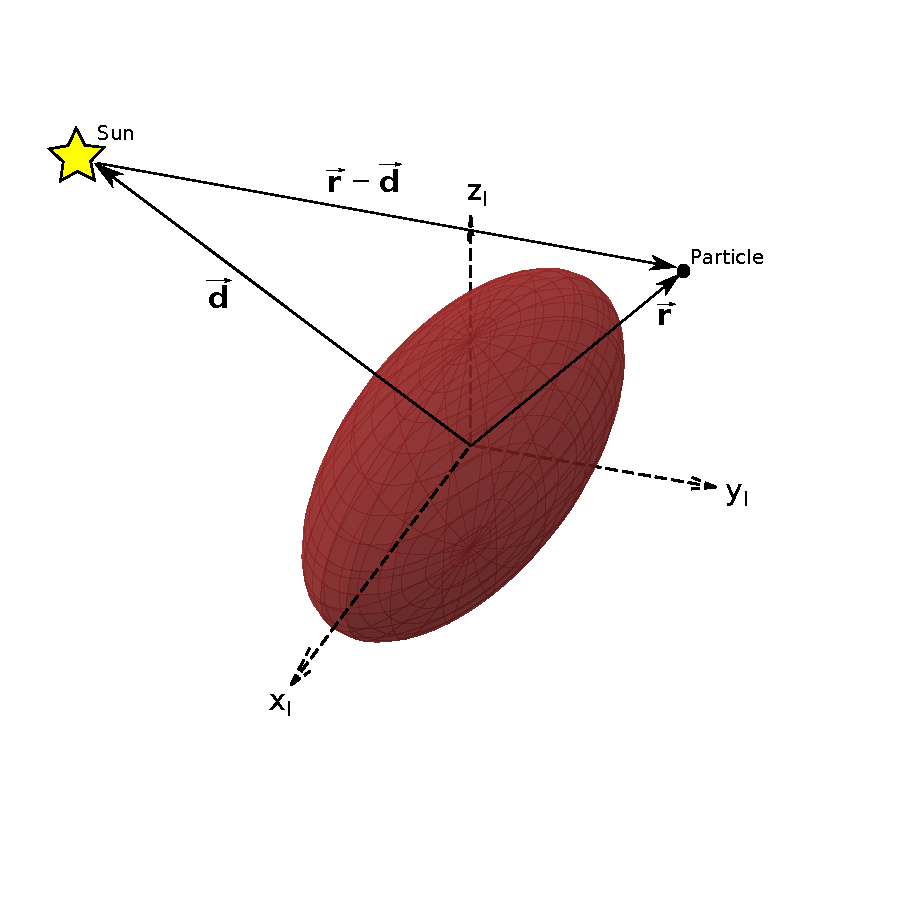
\includegraphics[width=\textwidth, height=0.35\textheight, keepaspectratio=true]{stbe_bodyframe_edit_2.pdf}
\caption{A schematic representing the orientation of position vectors of the Sun and the orbiting particle/regolith around the asteroid, in the \gls{AIF}. Diagram is not to scale and the rotation state of asteroid is such that the \gls{ARF} and \gls{AIF} are coinciding.}
\label{fig:stbe_bodyFrame}
\end{figure}
\FloatBarrier
%%%
Now the absolute gravitational acceleration, due to the Sun, experienced by the asteroid is given as follows \parencite{scheeresBook}:
%%%
\begin{align}
    \bv{a}_{abs, a} &= +\frac{\mu_S}{|\bv{d}|^3} (\bv{d})
    \label{eqn:stbe_asteroid_abs_acc}
\end{align}
%%%
where the definition of all variables is the same as that for \Cref{eqn:stbe_particle_abs_acc}. Thus, the perturbing acceleration acting on the particle due to the \gls{STBE} is the difference between the absolute accelerations experienced by the particle (\Cref{eqn:stbe_particle_abs_acc}) and the asteroid (\Cref{eqn:stbe_asteroid_abs_acc}) \parencite{scheeresBook}:
%%%
\begin{align}
    \bv{a}_{STBE} &= -\mu_S \left[ \frac{(\bv{r} - \bv{d})}{|\bv{r} - \bv{d}|^3} + \frac{\bv{d}}{|\bv{d}|^3} \right]
    \label{eqn:stbe_acc}
\end{align}
%%%
The perturbing acceleration in \Cref{eqn:stbe_acc} can be re-written in the form of a potential as follows \parencite{scheeresBook}:
%%%
\begin{align}
    \mathcal{R}_{STBE} &= \mu_S \left[\frac{1}{|\bv{r} - \bv{d}|} - \frac{\bv{d}\cdotp\bv{r}}{|\bv{d}|^3} \right]
    \label{eqn:stbe_potential} \\
    \bv{a}_{STBE} &= \frac{\delta \mathcal{R}_{STBE}}{\delta\bv{r}}
\end{align}
%%%
In \Cref{eqn:stbe_acc}, we can directly substitute the position vectors as defined in \gls{ARF} such that the acceleration term obtained is also in the \gls{ARF}. This is possible because the position magnitude terms would remain the same in either of the reference frames. Also, the rotation matrix $\phi_I^B$ multiplied either outside the square bracket or inside, in \Cref{eqn:stbe_acc}, with the two numerator terms would ultimately give the same result.
%%%
\begin{align}
    \ddot{\bv{d}} &= -\frac{\mu_S}{|\bv{d}|^3} (\bv{d})
    \label{eqn:sun_around_asteroid}
\end{align}
%%%
The apparent position of the Sun, relative to the asteroid, can be obtained in two ways. We could either numerically integrate the second order differential equation for the standard two-body problem as stated in \Cref{eqn:sun_around_asteroid} or solve, what is historically known as, the \textit{Kepler's problem}. We use the latter since the apparent position of the Sun can be obtained for any time value directly by using the Kepler's problem algorithm as stated by \cite{chobotovBook}. Although the Kepler's problem algorithm is not completely analytical and uses a numerical iteration method to solve for the true anomaly, it is relatively easier to use within the simulator than employing a numerical integrator to propagate the position from an initial condition for every time value. The algorithm for solving the Kepler's problem is not stated here for brevity; A detailed explanation for it is given by \cite{chobotovBook}.

\subsection{Solar Radiation Pressure (SRP)}
\label{subsec:srp}
With the heliocentric orbit of the asteroid, in addition to the \gls{STBE}, is a non-gravitational source of perturbation acting on an asteroid-orbiting particle, called \gls{SRP}. Momentum transfer takes place from the Solar photons that strike and recoil from the surface of the particle, which thus perturbs the orbital motion \parencite{scheeresBook}.
%
\newline\newline
%
We use a model for \gls{SRP} that assumes that the particle always presents a constant area to the impinging Solar photons and the area is perpendicular to the Sun-line. The total momentum transfer is modeled as Solar irradiance and reflection and the acceleration due to \gls{SRP} thus acts in a direction away from and along the Sun-line \parencite{scheeresBook}. This acceleration is given as follows:
%%%
\begin{align}
    \bv{a}_{SRP} &= -(1 + \rho) P_0 \cdotp \frac{A}{M} \cdotp \frac{(\bv{d} - \bv{r})}{|\bv{d} - \bv{r}|^3}
    \label{eqn:srp_acc}
\end{align}
%%%
where $\rho$ is the albedo of the particle; $P_0$ is a Solar constant whose value is $1.0\times10^{17}$ \si{\kilogram \metre \per \second \squared}; $A/M$ is the area-to-mass ratio of the particle and area refers to the cross-sectional area of the particle on which the Solar photons are striking; \bvt{d} is the distance vector from the asteroid to the Sun and \bvt{r} is the distance vector from the asteroid to the orbiting particle \parencite{scheeresBook}. The \gls{SRP} perturbing acceleration can be re-stated in terms of a perturbing potential as follows:
%%%
\begin{align}
    \mathcal{R}_{SRP} &= -(1 + \rho) P_0 \cdotp \frac{A}{M} \left[\frac{1}{|\bv{d}-\bv{r}|}\right]
    \label{eqn:srp_potential} \\
    \bv{a}_{SRP} &= \frac{\delta \mathcal{R}_{SRP}}{\delta \bv{r}}
\end{align}
%%%

\section{Perturbed Two-Body Problem}
\label{sec:2BP}
We have discussed the gravitational potential and the perturbations model to be used for our system, and now we'll present the \gls{EOM} that govern the motion of the lofted particle. Note that the \gls{CDE} potential model is defined for a body-fixed frame inherently which means the accelerations that we get out of it are directly defined for the \gls{ARF} frame. The same applies for the \gls{STBE} and \gls{SRP} perturbing accelerations. This is why we define the equations of motion too in the \gls{ARF} frame and transform the propagated state to the \gls{AIF} frame post-simulation.
%
\newline\newline
%
We use a Lagrangian approach to derive the \gls{EOM} because once the Lagrangian is formed, it becomes relatively easy to re-write the \gls{EOM} for a different frame of reference or a different set of coordinates by substituting the relevant transformation equations in the Lagrangian. It is formed as $L=T+\mathcal{U}$, where $T$ is the specific kinetic energy and $\mathcal{U}$ is the full potential of the system and they are given as follows \parencite{scheeresBook}:
%%%
\begin{align}
    T &= \frac{1}{2} \dot{\bv{r}}_I \cdotp \dot{\bv{r}}_I
    \label{eqn:lagrangian_kinetic_energy} \\
    \mathcal{U} &= U + \mathcal{R}_{STBE} + \mathcal{R}_{SRP}
    \label{lagrangian_potential}
\end{align}
%%%
where $\bv{r}_I$ is the position vector of the particle from the asteroid to the orbiting particle and expressed in the \gls{AIF}; $U$ is the \gls{CDE} gravity potential; $\mathcal{R}_{STBE}$ and $\mathcal{R}_{SRP}$ are the perturbing potentials for the Sun's third-body effect and radiation pressure respectively. The \gls{EOM} is then obtained from the following \parencite{scheeresBook}:
%%%
\begin{align}
    \frac{d}{dt} \left(\frac{\delta L}{\delta \dot{x}_i}\right) &= \frac{\delta L}{\delta x_i}
    \label{eqn:lagrange_general_form}
\end{align}
%%%
where $(x_i, \dot{x}_i)$ are the position and velocity vector components. We will now evaluate \Cref{eqn:lagrange_general_form} for our particular case by first re-stating the Lagrangian with vectors expressed in the \gls{ARF}. With $(\bv{q}, \dot{\bv{q}})$ denoting the \gls{ARF} position and velocity vectors respectively, the position vector in the \gls{AIF} is related to the \gls{ARF} as $\bv{r} = \phi_B^I \bv{q}$ and the velocity is related as $\dot{\bv{r}} = \phi_I^B \cdotp (\dot{\bv{q}} + \bv{\omega} \times \bv{q})$. With these definitions, the Lagrangian is re-written as follows:
%%%
\begin{align}
    L &= (\dot{\bv{q}} + \bv{\omega} \times \bv{q}) \cdotp (\dot{\bv{q}} + \bv{\omega} \times \bv{q}) + \mathcal{U}(\bv{q})
    \label{eqn:lagrange_arf}
\end{align}
%%%
where the transformation matrix $\phi_B^I$ preserves \footnote{For two vectors \bvt{u} and \bvt{v}, and an orthogonal matrix $Q$, $\bv{u} \cdotp \bv{v} = (Q\bv{u}) \cdotp (Q\bv{v})$} the dot product, as it is orthogonal, and hence is excluded from the equation. The derivative on the right hand side of \Cref{eqn:lagrange_general_form}, directly in vector form, is evaluated as follows:
%%%
\begin{align}
    \frac{\delta L}{\delta \bv{q}} &= \frac{1}{2} \left[ 2 \cdotp (\dot{\bv{q}} + \bv{w} \times \bv{q}) \cdotp (\bv{\omega} \times \bv{1} + \bv{q} \times {\bv{0}}) \right] + \frac{\delta \mathcal{U}}{\delta \bv{q}} \\
    &= \dot{\bv{q}} \cdotp (\bv{\omega} \times \bv{1}) + (\bv{\omega} \times \bv{q}) \cdotp (\bv{\omega} \times \bv{1}) + \frac{\delta \mathcal{U}}{\delta \bv{q}} \\
    &= (\dot{\bv{q}} \times \bv{\omega}) \cdotp \bv{1} + \bv{1} \cdotp ((\bv{\omega} \times \bv{q}) \times \bv{\omega}) + \frac{\delta \mathcal{U}}{\delta \bv{q}} \\
    &= -(\bv{\omega} \times \dot{\bv{q}}) - (\bv{\omega} \times (\bv{\omega} \times \bv{q})) + \frac{\delta \mathcal{U}}{\delta \bv{q}}
    \label{eqn:lagrangian_RHS}
\end{align}
%%%
where \bvt{1} and \bvt{0} are vectors of ones and zeros respectively and all other terms have been defined previously. The left hand side of \Cref{eqn:lagrange_general_form} is evaluated as follows:
%%%
\begin{align}
    \frac{\delta L}{\delta \dot{\bv{q}}} &= \dot{\bv{q}} + (\bv{\omega} \times \bv{q}) \\
    \frac{d}{dt}\left( \frac{\delta L}{\delta \dot{\bv{q}}} \right) &= \ddot{\bv{q}} + \bv{\omega} \times \dot{\bv{q}}
    \label{eqn:lagrangian_LHS}
\end{align}
%%%
Thus, by substituting \Cref{eqn:lagrangian_LHS,eqn:lagrangian_RHS} into \Cref{eqn:lagrange_general_form}, we get the final equations of motion as follows:
%%%
\begin{align}
    \ddot{\bv{q}} + 2 \cdotp \bv{\omega} \times \dot{\bv{q}} + (\bv{\omega} \times (\bv{\omega} \times \bv{q})) &= \frac{\delta \mathcal{U}}{\delta \bv{q}} \\
    &= \frac{\delta U(\bv{q})}{\delta \bv{q}} + \frac{\delta \mathcal{R}_{STBE}}{\delta \bv{q}} + \frac{\delta \mathcal{R}_{SRP}}{\delta \bv{q}}
    \label{eqn:lagrangian_potential_eval} \\
    \ddot{\bv{q}} + 2 \cdotp \bv{\omega} \times \dot{\bv{q}} + (\bv{\omega} \times (\bv{\omega} \times \bv{q})) &= \frac{\delta U(\bv{q})}{\delta \bv{q}} + \bv{a}_{STBE} + \bv{a}_{SRP}
    \label{eqn:p2bp}
\end{align}
%%%
In \Cref{eqn:lagrangian_potential_eval}, the first term denotes the acceleration due to gravity, and the second and the third term denote the perturbing accelerations. \Cref{eqn:p2bp} is thus the final equation of motion used in this thesis.

\section{Particle Initial Conditions}
\label{sec:init_conditions}
The \gls{EOM} established in the previous section are difficult to solve analytically and hence we make use of a numerical integrator to propagate the state vector of an orbiting particle in time. To do this, we need to establish robust methods for providing initial conditions. These initial conditions basically form the state vector with which the particle is lofted from the surface of an asteroid.

\subsection{Launch Location}
\label{subsec:launch_location}
This section will present a method to efficiently calculate the launch location of a particle, in the form of a Cartesian position vector from the centre of the asteroid. The formulation is such that the resulting position vector will always point to a location on the surface of the asteroid.
%
\newline\newline
%
Consider the equation for the ellipsoid given as follows:
%%%
\begin{align}
    \frac{x^2}{\alpha^2} + \frac{y^2}{\beta^2} + \frac{z^2}{\gamma^2} &= 1
    \label{eqn:launch_loc_ellipsoid_eqn_cartesian}
\end{align}
%%%
where $(x,y,z)$ is the coordinate of any point \emph{on} the surface. An alternate way of writing \Cref{eqn:launch_loc_ellipsoid_eqn_cartesian}, in vector format, is given as follows:
%%%
\begin{align}
    \bv{r}.E.\bv{r} &= 1
    \label{eqn:launch_loc_ellipsoid_eqn_vectorForm} \\
    E &=
    \begin{bmatrix}
        1/\alpha^2 & 0 & 0 \\
        0 & 1/\beta^2 & 0 \\
        0 & 0 & 1/\gamma^2
    \end{bmatrix}
\end{align}
%%%
where \bvt{r} is a general position vector expressed in the \gls{ARF} and ($\alpha, \beta, \gamma$) are the semi-major axes of the triaxial ellipsoid model of the asteroid. Continuing with \Cref{eqn:launch_loc_ellipsoid_eqn_vectorForm}:
%%%
\begin{align}
    \bv{r}.\bv{r} &= \frac{1}{E} \\
    r^2 &= \frac{1}{\buvec{u}.E.\buvec{u}}
    \label{eqn:launch_loc_r_square}
\end{align}
%%%
where $\buvec{u}$ is a unit vector expressed in \gls{ARF}, pointing in the direction of the launch location from the asteroid's centre, with components $(u_x, u_y, u_z)$. The unit vector can be stated in terms of the latitude $(\delta)$ and longitude $(\lambda)$ of the launch point as follows:
%%%
\begin{align}
    \buvec{u} &= \cos\delta \cos\lambda \buvec{x} + \cos\delta \sin\lambda \buvec{y} + \sin\delta \buvec{z}
\end{align}
%%%
where $(\buvec{x},\buvec{y},\buvec{z})$ are the basis vectors forming the \gls{ARF}. Thus, \Cref{eqn:launch_loc_r_square} can be written as:
%%%
\begin{align}
    r^2 &= \frac{1}{ (u_x^2/\alpha^2) + (u_y^2/\beta^2) + (u_z^2/\gamma^2) }
    \label{eqn:launch_loc_r_square_expanded}
\end{align}
%%%
The final position vector to the launch location, from the origin of \gls{ARF} or the asteroid's centre, is given as follows:
%%%
\begin{align}
    \bv{r}_s &= r\buvec{u}
    \label{eqn:launch_vector}
\end{align}
%%%
where $r$ is obtained from \Cref{eqn:launch_loc_r_square_expanded}. Thus, just by specifying the latitude and longitude of any desired launch point, the position vector to it is obtained. This, thus, acts as the initial position state of the particle.

\subsection{Launch Velocity}
\label{subsec:launch_velocity}
Once we know the position of the particle, we need to provide an initial velocity to launch it into an orbit around the asteroid. But this has to do much more than just providing a velocity magnitude. The velocity magnitude is accompanied by a launch direction which is defined by two angles, namely, \emph{Launch Azimuth} ($\eta$) and \emph{Launch Declination} ($\chi$).
%
\newline\newline
%
These angles can be understood as follows. Suppose you are standing on the surface of an asteroid and you throw a ball. Now the ball will be associated with a velocity vector and if we take the projection of this vector onto the local surface, then the angle between this projection and the local direction to the North pole of the asteroid is defined as the launch azimuth. The angle that the velocity vector itself makes with the local normal is then defined as the launch declination. By keeping a constant angle of declination and varying the launch azimuth from \SI{0}{\degree} to \SI{360}{\degree}, we can create a cone of particles, thus replicating how impact ejecta would launch out. An example of this is given in \Cref{fig:longest_edge_velocity_vector_cone}.
%%%
\begin{figure}[htb]
\centering
\captionsetup{justification=centering}
\subfloat[]{
    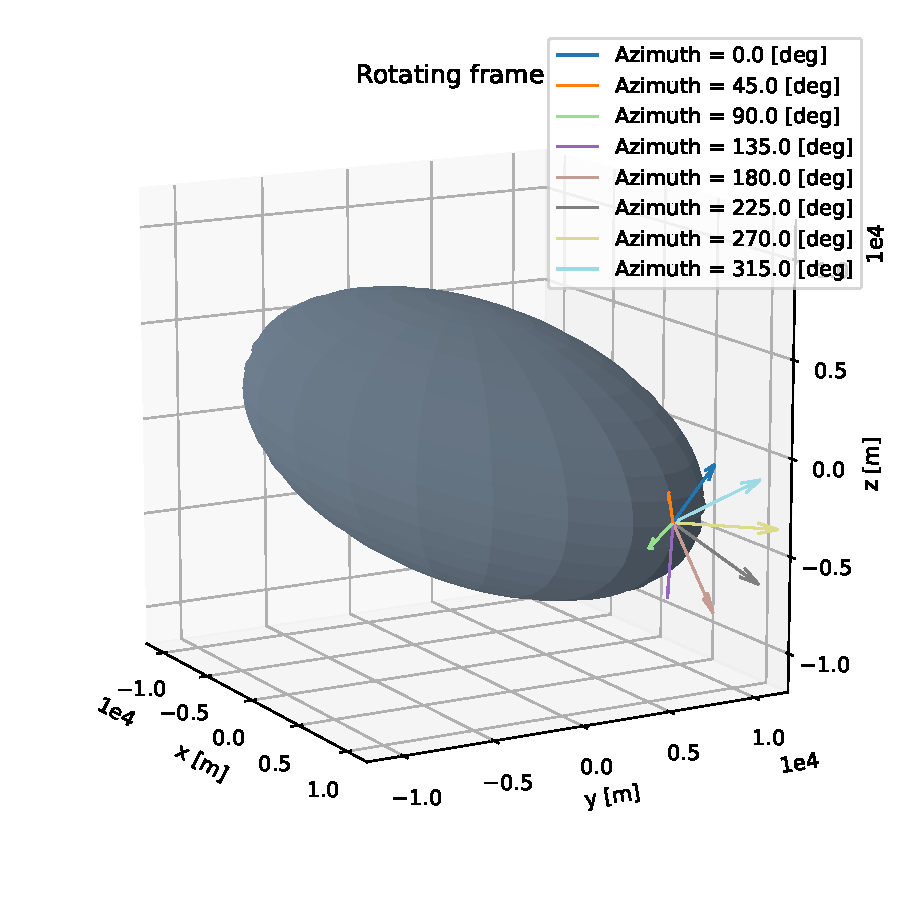
\includegraphics[width=\textwidth, height=0.5\textheight, keepaspectratio=true]{longest_edge_ARF_velocity_vectors_cone.pdf}
    \label{fig:longestEdge_velocity_vector_cone_1}
}

\subfloat[]{
    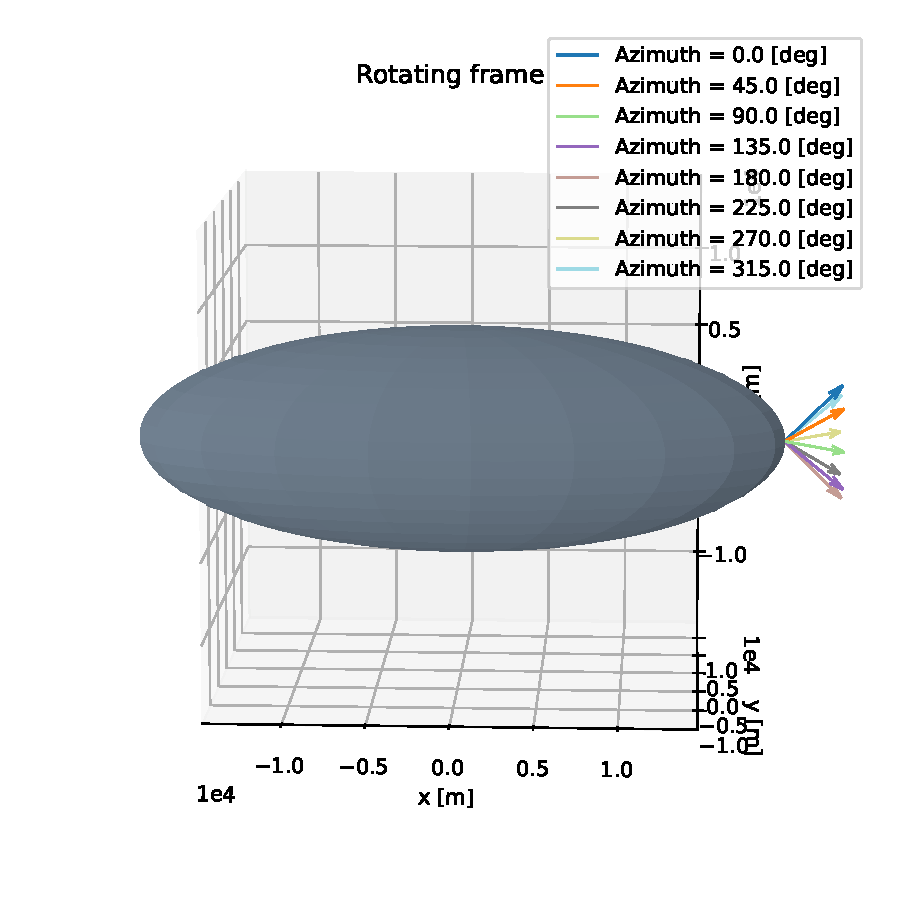
\includegraphics[width=\textwidth, height=0.5\textheight, keepaspectratio=true]{velocity_vector_ARF_lateral_view.pdf}
    \label{fig:longestEdge_velocity_vector_cone_2}
}
\caption{Various velocity vectors depicted at the longest edge of the ellipsoid shaped asteroid i.e. for a launch location longitude and latitude of \SI{0}{\degree}. \protect\Cref{fig:longestEdge_velocity_vector_cone_1} depicts the front view of multiple velocity vectors spaced at \SI{45}{\degree} azimuth from each other and at a constant declination of \SI{45}{\degree}. All vectors are expressed in the rotating frame or the \gls{ARF}. \protect\Cref{fig:longestEdge_velocity_vector_cone_2} depicts the lateral view of the same velocity vectors.}
\label{fig:longest_edge_velocity_vector_cone}
\end{figure}
\FloatBarrier
%%%
We will now discuss how the velocity vectors are formed in practice. Consider the equation for a triaxial ellipsoid given in \Cref{eqn:launch_loc_ellipsoid_eqn_cartesian}. Now for any given point $(x,y,z)$ on the surface of the ellipsoid, the normal vector ($\bv{n}$) (and subsequently the unit normal vector ($\buvec{n}$)) to it is found by taking the gradient of \Cref{eqn:launch_loc_ellipsoid_eqn_cartesian}:
%%%
\begin{align}
    \bv{n} &= \frac{2x}{\alpha^2}\buvec{i} + \frac{2y}{\beta^2}\buvec{j} + \frac{2z}{\gamma^2}\buvec{k}
    \label{eqn:surface_normal_vector} \\
    \buvec{n} &= \frac{\bv{n}}{|\bv{n}|}
    \label{eqn:unit_normal}
\end{align}
%%%
where both \bvt{n} and $\buvec{n}$ are expressed in the \gls{ARF}, whose basis vectors are denoted here as ($\buv{i},\buv{j},\buv{k}$). Note that since the body in question is not a sphere, the normal vector at the launch location and the radial unit vector $\buv{R}$ (from the centre of the ellipsoid to the launch location) may not always coincide. Now that we know the unit normal vector to the launch location, we need to find the local North direction. This is done by performing the following calculations successively:
%%%
\begin{align}
    \buv{R} &= \frac{\bv{r}_s}{|\bv{r}_s|} \\
    \buv{T} &= \frac{\buv{R} \times \buv{k}}{|\buv{R} \times \buv{k}|} \\
    \buv{x} &= \frac{\buv{T} \times \buv{n}}{|\buv{T} \times \buv{n}|} \\
    \label{eqn:surface_frame_xBasis}
\end{align}
%%%
where $\bv{r}_s$ is the position vector to the launch location from the centre of the asteroid; $\buv{T}$ is the tangential unit vector (tangential to the local surface at the local point); $\buv{x}$ is the unit vector that is pointing towards the local North. This formulation works for any point on the surface of the asteroid to give the local North's direction except for the two poles and as such an alternative definition for them has to be used which will be defined later. Note that all the unit vectors discussed so far are expressed in the \gls{ARF}.
%
\newline\newline
%
$\buv{x}$ is also viewed as the x-axis basis vector for a frame of reference fixed and centered at the launch location. This frame of reference is termed as the \gls{SF}. Note that the \gls{SF} is not used to define the orbital motion of the regolith and hence it is not one of the standard reference frames. This is why it wasn't mentioned in \Cref{sec:reference_frames} and is only defined here since it's use is only for obtaining the velocity vector. The z-axis of \gls{SF} is defined in the direction of the unit normal vector at the launch location and the y-axis is obtained by following the right-hand rule to form the orthogonal frame. The \gls{SF} is shown in \Cref{fig:surface_frame}.
%
\newline\newline
%
Note that the basis vectors of the \gls{SF} are expressed in the \gls{ARF} and thus their components are defined as follows:
%%%
\begin{align}
    \buv{x} &= x_1\buv{i} + x_2\buv{j} + x_3\buv{k}
    \label{eqn:sf_xbasis_exp} \\
    \buv{y} &= y_1\buv{i} + y_2\buv{j} + y_3\buv{k}
    \label{eqn:sf_ybasis_exp} \\
    \buv{z} &= z_1\buv{i} + z_2\buv{j} + z_3\buv{k}
    \label{eqn:sf_zbasis_exp}
\end{align}
%%%
Then the velocity vector components in \gls{ARF} are obtained as follows:
%%%
\begin{align}
    v_x &= V . \left[ x_1 \cos\eta \sin\chi + y_1 \sin\eta \sin\chi + z_1 \cos\chi \right]
    \label{eqn:xVelocity} \\
    v_y &= V . \left[ x_2 \cos\eta \sin\chi + y_2 \sin\eta \sin\chi + z_2 \cos\chi \right]
    \label{eqn:yVelocity} \\
    v_z &= V . \left[ x_3 \cos\eta \sin\chi + y_3 \sin\eta \sin\chi + z_3 \cos\chi \right]
    \label{eqn:zVelocity}
\end{align}
%%%
where $V$ is the magnitude of the velocity chosen manually at the start of the simulation. Thus in this manner, and for the same velocity magnitude, we can simulate particles being launched in different directions from the same launch location, which in turn helps us understand the role of launch direction in the final fate of ejecta.
%%%
\begin{figure}[htb]
\centering
\captionsetup{justification=centering}
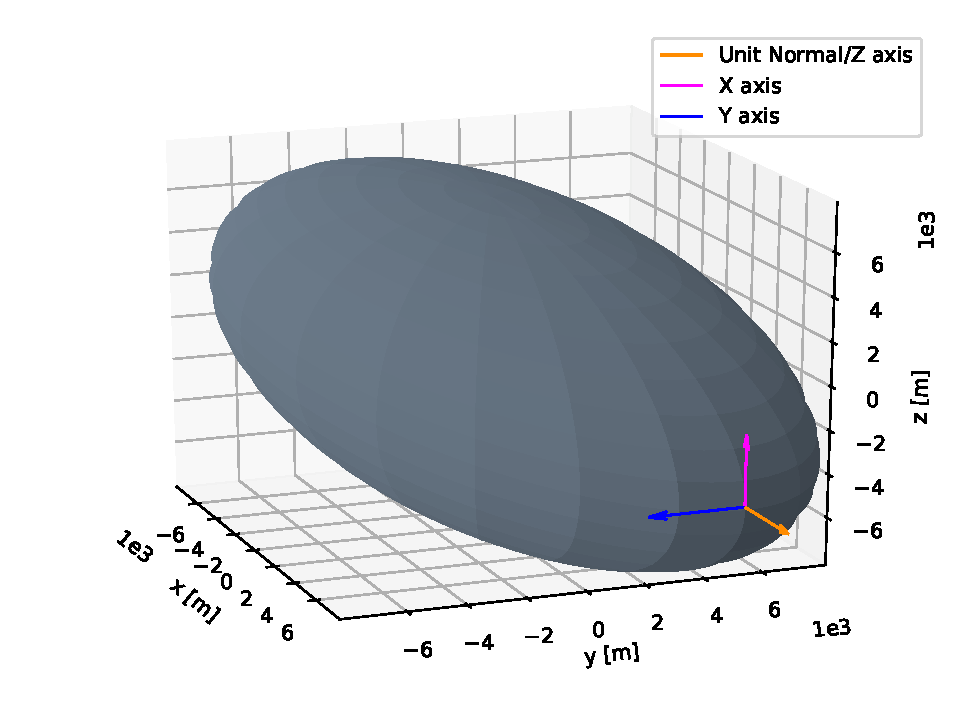
\includegraphics[width=\textwidth, height=0.4\textheight, keepaspectratio=true]{surfaceFrame_longestEdge.pdf}
\caption{An example of the \gls{SF} at the launch location of latitude and longitude \SI{0}{\degree} i.e. the longest edge of the asteroid. The x-axis points to the local North; z-axis is in the direction of the unit normal vector at the launch location; and finally the y-axis completes right-hand rule orthogonal frame.}
\label{fig:surface_frame}
\end{figure}
\FloatBarrier
%%%
As said earlier, the x-basis vector for the \gls{SF} can not be defined by the method described previously for launch locations on the two poles of the asteroid. Hence we use two alternate definitions for the x-basis vector in those scenarios however all other computations remain the same as described before. If the launch location is the North pole, then the x-basis vector of the \gls{SF} is defined as $\buv{x}=[1, 0, 0]$ and for South pole it is defined as $\buv{x}=[-1, 0, 0]$.

\section{Non-conservative Guarantee Escape Speed}
\label{sec:escape_speed_derivation}
Up until now we discussed the dynamics involved with the particle motion around an asteroid and we also devised methods to launch regolith from the surface into an orbit. It was mentioned earlier that the thesis has employed a full numerical simulation approach to the problem at hand, but while doing that we did attempt at finding a new analytical method to determine a non-conservative guarantee escape speed.
%
\newline\newline
%
The conservative guarantee escape speed method is obtained by making use of the maximum gravitational potential, between the actual potential of the irregular body and an equivalent point mass potential, at the location of the launch of the particle. If the launch speed is above the conservative guarantee escape speed, then the particle will escape immediately after launch. The conservative guaranteed escape speed method works best for uniform gravity field models, as we'll see later in \Cref{subsec:nonconservative}, but fails when one accounts for non-uniform gravity field models such as the \gls{CDE} model.
% This method however, does not account for the cases which result in an escape situation after completing one or more orbital revolutions around the asteroid or basically the cases where the launch speed is below the conservative guarantee escape speed and still result in an escape scenario. The idea of developing a new analytical method stems from this problem and we call it the non-conservative guarantee escape speed since we aim to account for those cases as well where the escape does not happen immediately.
%
\newline\newline
%
We will first understand how the conventional guarantee escape speed is obtained since it will help us in understanding the method for the non-conventional guarantee escape speed later on. The inertial velocity of a particle which is resting on an asteroid's surface is given as $\bv{v}_I = \bv{\omega} \times \bv{r}$, where \bvt{r} is the location to the particle from the centre of the asteroid. The resulting vector is pointing outwards from the asteroid if the launch location is on the leading edge of the asteroid and inwards if the launch location is on the trailing edge of the asteroid \parencite{scheeresBook}. The idea is easily depicted in \Cref{fig:conservative_escape_speed_leading_trailing_edges}.
%%%
\begin{figure}[htb]
\centering
\captionsetup{justification=centering}
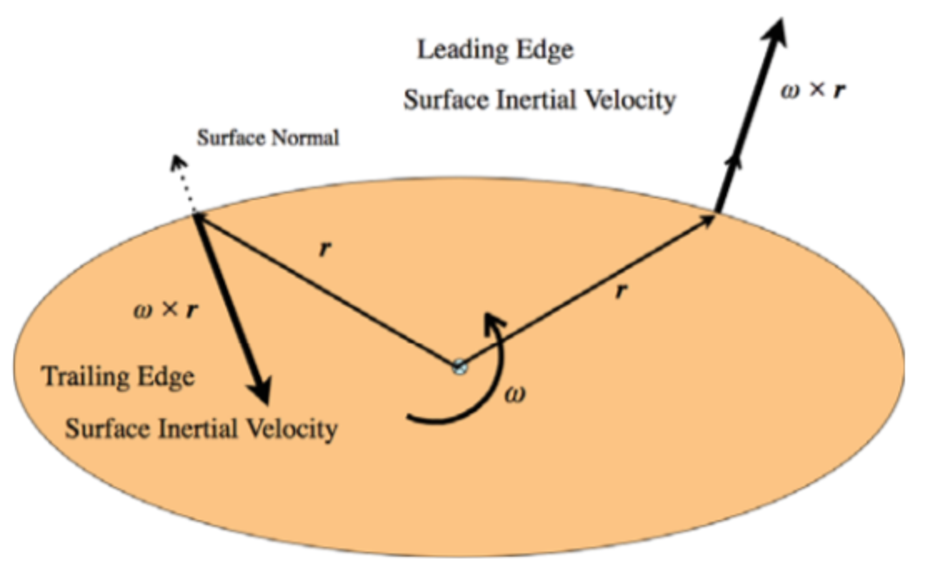
\includegraphics[width=\textwidth, height=0.3\textheight, keepaspectratio=true]{leading_trailing_edge.pdf}
\caption{Schematic for inertial velocity at the surface for different launch locations \parencite{scheeresBook}.}
\label{fig:conservative_escape_speed_leading_trailing_edges}
\end{figure}
\FloatBarrier
%%%
The idea now is to provide an additional launch speed, for instance in the normal direction, that would result in an escape scenario for the particle. The inertial velocity can then be expressed as follows \parencite{scheeresBook}:
%%%
\begin{align}
    \bv{v}_I &= v_{e}\buv{n} + \bv{\omega} \times \bv{r}
    \label{eqn:conservative_inertial_escape}
\end{align}
%%%
where $v_e\buv{n}$ is the velocity, expressed in \gls{ARF}, with which a particle is launched in the normal direction such that the particle is on an escape trajectory. All other terms have been defined previously. The conservative approach is to equate $\bv{v}_I$ to $\sqrt{2U_{max}}$ where $U_{max} = max[U(\bv{r}), \mu/\bv{r}]$ \parencite{scheeresBook}. \Cref{eqn:conservative_inertial_escape} can then be re-written as follows:
%%%
\begin{align}
    \sqrt{2U_{max}} &= v_{e}\buv{n} + \bv{\omega} \times \bv{r} \\
    2U_{max} &= v_e^2 + (\bv{\omega} \times \bv{r})^2 + 2 v_e (\buv{n} \cdotp (\bv{\omega} \times \bv{r}))
    \label{eqn:conservative_quadratic}
\end{align}
%%%
\Cref{eqn:conservative_quadratic} is a quadratic equation in $v_e$ and can be solved as follows:
%%%
\begin{align}
    v_e &= \frac{-2(\buv{n} \cdotp (\bv{\omega} \times \bv{r})) \pm \sqrt{4 (\buv{n} \cdotp (\bv{\omega} \times \bv{r}))^2 + 4 (2U_{max}) - 4(\bv{\omega} \times \bv{r})^2}}{2} \\
    v_e &= -(\buv{n} \cdotp (\bv{\omega} \times \bv{r})) \pm \sqrt{(\buv{n} \cdotp (\bv{\omega} \times \bv{r}))^2 + 2U_{max} - (\bv{\omega} \times {\bv{r}})^2}
\end{align}
%%%
Since the speed can't be negative, the formula is re-written as:
%%%
\begin{align}
    v_e &= -(\buv{n} \cdotp (\bv{\omega} \times \bv{r})) + \sqrt{(\buv{n} \cdotp (\bv{\omega} \times \bv{r}))^2 + 2U_{max} - (\bv{\omega} \times {\bv{r}})^2}
    \label{eqn:conservative_escape_speed}
\end{align}
%%%
\Cref{eqn:conservative_escape_speed} thus gives the conservative escape speed, expressed in the \gls{ARF}, for a particle launched in the normal direction. The equation is equally applicable for a particle launched in any general direction as well by substituting $\buv{n}$ with the unit vector for the direction in which the launch takes place. Thus if a particle is launched with a velocity above or equal to the one mentioned in \Cref{eqn:conservative_escape_speed}, then it would result in a guaranteed escape situation.
%
\newline\newline
%
Now for a non-conservative approach, we will not use $\bv{v}_I = \sqrt{2U_{max}}$ to get a guaranteed escape launch speed. We will derive an alternate relation for $\bv{v}_I$ first and then later on substitute it back into \Cref{eqn:conservative_escape_speed} in place of $2U_{max}$ to get the non-conservative guaranteed escape launch speed.
%
\newline\newline
%
Consider the \gls{EOM} mentioned in \Cref{eqn:p2bp}, with the exception that we only consider the gravitational potential and remove all external perturbations on the left hand side of the equation. These equations do not have an explicit dependence on time which means that the Jacobian for the system exists and is conserved \parencite{scheeresBook}. The Jacobian, expressed in the \gls{ARF}, is given as follows \parencite{scheeresBook}:
%%%
\begin{align}
    J &= \frac{1}{2} v_B^2 - \frac{1}{2} \omega^2(x^2 + y^2) - U(\bv{r})
    \label{eqn:jacobian}
\end{align}
%%%
where $v_B$ is the velocity of the particle in the \gls{ARF}; $\omega$ is the magnitude of the angular velocity of the rotating asteroid and is along the z-axis of the \gls{ARF}; $(x,y)$ are the x-y coordinate of the orbiting particle; $U(\bv{r})$ is the small-body gravitational potential, which in our case is the \gls{CDE} potential model. From transport theorem, we use the relation between an inertial velocity and the rotating frame velocity:
%%%
\begin{align}
    \bv{v}_B &= \bv{v}_I - (\bv{\omega} \times \bv{r}) \\
    v_B^2 &= v_I^2 + (\bv{\omega} \times \bv{r})^2 - 2 \bv{v}_I \cdotp (\bv{\omega} \times \bv{r}) \\
    v_B^2 &= v_I^2 + (\bv{\omega} \times \bv{r})^2 - 2 \bv{\omega} \cdotp (\bv{r} \times \bv{v}_I) \\
    v_B^2 &= v_I^2 + (\bv{\omega} \times \bv{r})^2 - 2 \bv{\omega} \cdotp \bv{H}
    \label{eqn:arf_velocity_modified_with_H}
\end{align}
%%%
where \bvt{H} is the angular momentum of the orbiting particle. We substitute \Cref{eqn:arf_velocity_modified_with_H} back into \Cref{eqn:jacobian} to get the following relation:
%%%
\begin{align}
    J &= \frac{1}{2} v_I^2 - \bv{\omega} \cdotp \bv{H} - U(\bv{r})
    \label{eqn:jacobian_mod}
\end{align}
%%%
Considering that after launch the particle is on a parabolic trajectory such that it barely escapes then in such a case the energy of the particle would be 0 which reduces the Jacobian to $J_{\infty} = -\bv{\omega} \cdotp \bv{H}_{\infty}$. Now at the instance of the launch, the Jacobian is expressed as follows:
%%%
\begin{align}
    J_0 &= \frac{1}{2} v_{I_0}^2 - \bv{\omega} \cdotp \bv{H}_0 - U(\bv{r}_0)
    \label{eqn:jacobian_t0}
\end{align}
%%%
Since the Jacobian is conserved, $J_0 = J_{\infty}$, which means we can write the following relation:
%%%
\begin{align}
    \frac{1}{2} v_{I_0}^2 - \bv{\omega} \cdotp \bv{H}_0 - U(\bv{r}_0) &= -\bv{\omega} \cdotp \bv{H}_{\infty}
    \label{eqn:jacobian_equate}
\end{align}
%%%
For parabolic trajectories, the angular momentum magnitude is expressed in terms of the semi-latus rectum and the gravitational parameter of the central body as $H = \sqrt{\mu 2q}$ where $q$ is the periapsis distance \parencite{schaub2003Book}. Also the angle between the angular momentum vector and the asteroid's rotation vector is the orbit inclination ($i$) and with these new definitions, \Cref{eqn:jacobian_equate} is re-written as follows:
%%%
\begin{align}
    \frac{1}{2} v_{I_0}^2 - \bv{\omega} \cdotp \bv{H}_0 - U(\bv{r}_0) &= -\omega \cos(i) \sqrt{2\mu q_{\infty}}
    \label{eqn:jacobian_equate_cosi}
\end{align}
%%%
We will consider only equatorial orbits for now and hence \Cref{eqn:jacobian_equate_cosi} can be stated as simply:
%%%
\begin{align}
    \frac{1}{2} v_{I_0}^2 - \bv{\omega} \cdotp \bv{H}_0 - U(\bv{r}_0) &= -\omega \sqrt{2\mu q_{\infty}} \\
    \frac{1}{2} v_{I_0}^2 - \bv{\omega} \cdotp (\bv{r}_0 \times \bv{v}_{I_0}) - U(\bv{r}_0) &= -\omega \sqrt{2\mu q_{\infty}}
    \label{eqn:jacobian_equate_equatorial}
\end{align}
%%%
Note we can write $H_0 = \bv{r}_0 \times \bv{v}_{I_0}$, where $\bv{r_0}$ is expressed in \gls{ARF}, since at time $t = 0$ both \gls{ARF} and \gls{AIF} are aligned which means that $\bv{r}_{I_0} = \bv{r}_{B_0}$. The intent now is to solve for $v_{I_0}$ from \Cref{eqn:jacobian_equate_equatorial}, which is the inertial velocity at launch that eventually leads to an escape scenario.
%%%
\begin{figure}[htb]
\centering
\captionsetup{justification=centering}
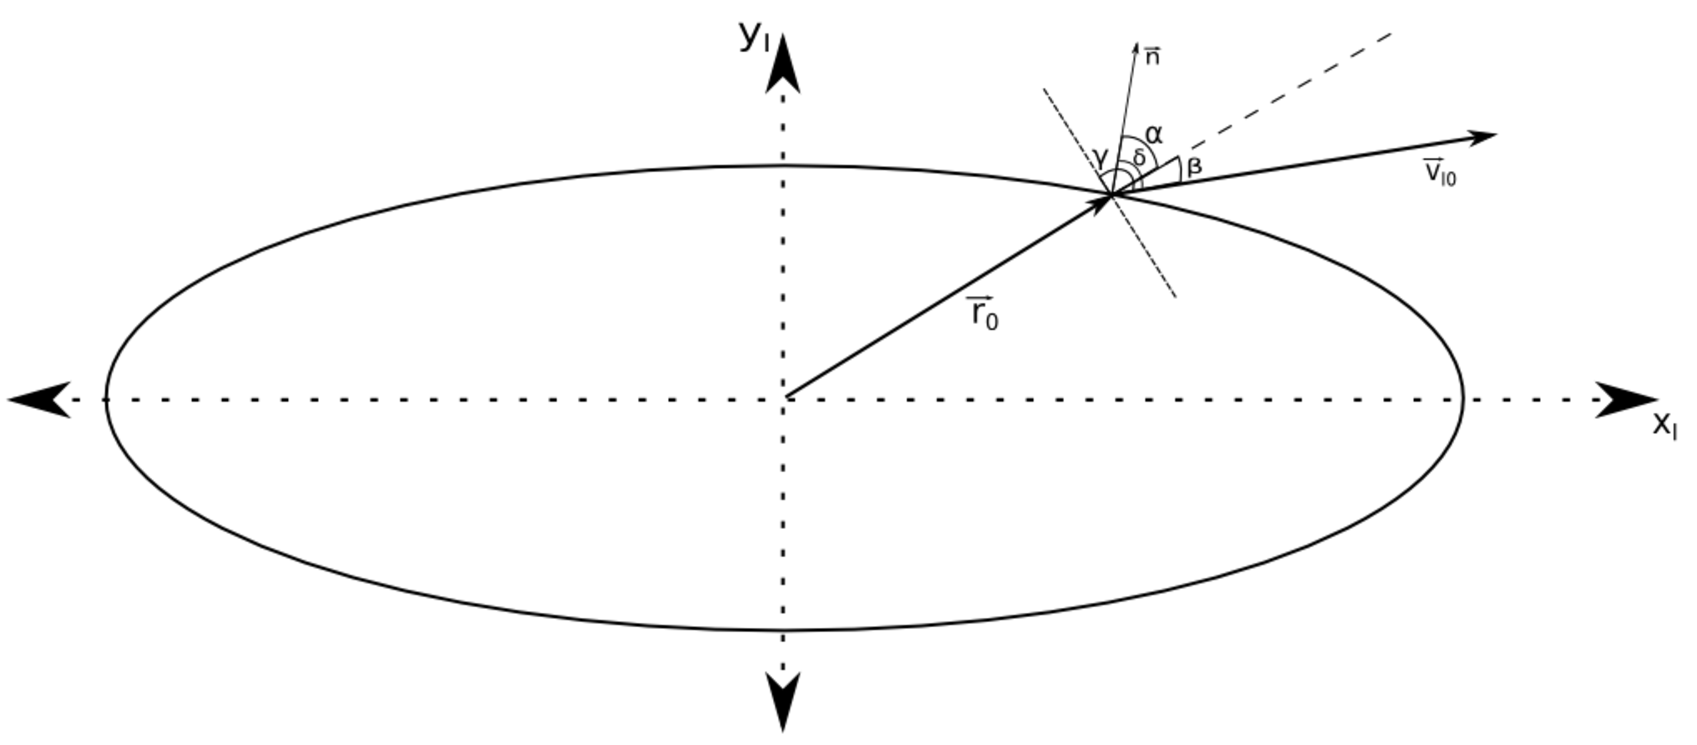
\includegraphics[width=\textwidth, height=0.3\textheight, keepaspectratio=true]{non_conservative_escape_velocity_angles.pdf}
\caption{General angle definitions for velocity vector with position and normal vector at the launch location.}
\label{fig:velocity_vector_angles}
\end{figure}
\FloatBarrier
%%%
We need to evaluate the second term on the left hand side of \Cref{eqn:jacobian_equate_equatorial} using the angle definitions given in \Cref{fig:velocity_vector_angles}. In that, $\gamma$ is the angle between the velocity vector and the plane perpendicular to the position vector; $\delta$ is the launch declination angle as explained in \Cref{subsec:launch_velocity}; $\alpha$ is the angle between the normal vector and the position vector direction and finally, $\beta$ is the angle between the velocity vector and the position vector direction. Using these definitions, the cross product in \Cref{eqn:jacobian_equate_equatorial} is evaluated as follows:
%%%
\begin{align}
    \bv{\omega} \cdotp (\bv{r}_0 \times \bv{v}_{I_0}) &= \bv{\omega} \cdotp (r_0 v_{I_0} \sin(\beta) \buv{h}) \\
    % &= \omega r_0 v_{I_0} \sin(-(90 - \gamma)) \\
    % &= -\omega r_0 v_{I_0} \cos(\gamma) \\
    % &= -\omega r_0 v_{I_0} \cos(90 - \alpha + \delta) \\
    % &= -\omega r_0 v_{I_0} \sin(\alpha - \delta) \\
    &= (r_0 v_{I_0} \sin(\delta - \alpha)) \bv{\omega} \cdotp \buv{h}
    \label{eqn:cross_product_eval}
\end{align}
%%%
where $\buv{h}$ specifies the direction of the cross product, i.e. the angular momentum vector $\bv{H}_0$. The angle definitions given in \Cref{fig:velocity_vector_angles} remains valid even for a launch location at the trailing edge of the asteroid and hence the angular definitions remain generalized. In addition to having an equatorial orbit, we can further simplify \Cref{eqn:cross_product_eval} by keeping the launch site at the longest edge of the ellipsoid which means that we can make $\alpha=0$. Thus \Cref{eqn:jacobian_equate_equatorial} can be re-written as:
%%%
\begin{align}
    \frac{1}{2} v_{I_0}^2 - (r_0 v_{I_0} \sin(\delta)) \bv{\omega}\cdotp\buv{h} - U(\bv{r}_0) &= -\omega \sqrt{2\mu q_{\infty}}
    \label{eqn:jacobian_equate_equatorial_mod}
\end{align}
%%%
\Cref{eqn:jacobian_equate_equatorial_mod} is a quadratic equation in $v_{I_0}$ which is solved to provide the following solution:
%%%
\begin{align}
    v_{I_0} &= (r_0 \sin\delta) \bv{\omega}\cdotp\buv{h} \pm \sqrt{((r_0 \sin\delta)\bv{\omega}\cdotp\buv{h})^2 + 2U - 2\omega\sqrt{2\mu q_\infty}}
    \label{eqn:non_conservative_inertial_guaranteed_escape_speed}
\end{align}
%%%
Thus instead of using $v_{I_0} = \sqrt{2U_{max}}$ in \Cref{eqn:conservative_quadratic}, we use the formula in \Cref{eqn:non_conservative_inertial_guaranteed_escape_speed} which leads to modifying \Cref{eqn:conservative_escape_speed} as follows:
%%%
\begin{align}
    v_e &= -(\buv{d} \cdotp (\bv{\omega} \times \bv{r})) + \sqrt{(\buv{d} \cdotp (\bv{\omega} \times \bv{r}))^2 + v_{I_0}^2 - (\bv{\omega} \times {\bv{r}})^2}
    \label{eqn:nonconservative_escape_speed}
\end{align}
%%%
where instead of using $\buv{n}$ we use the unit vector $\buv{d}$, representing a general direction of launch and not just the normal direction. Note that \Cref{eqn:jacobian_equate_equatorial_mod,eqn:non_conservative_inertial_guaranteed_escape_speed} are valid only for the launch location at the longest edge of the ellipsoid. We simplified the equations by making $\alpha=0$ so that testing this approach for a non-conservative guaranteed escape speed can be made easy, however the approach can be generalized by using a non-zero value for $\alpha$ in \Cref{eqn:cross_product_eval} as well.

\section{Conclusion}
\label{sec:dynamics_conclusion}
